\setcounter{chapter}{9}

\chapter{多元函数的导数及其应用}

本章也可以称为多元函数微分学,其中包含了对一元函数微分学中相关概念
的推广。需要注意的是,和向量值函数不同,这种推广并没有那么
“顺畅”,正因为如此,在理解和应用多元函数导数和微分的性质时,需要特别
留意一些与此前一元函数导数和微分不同的地方。

通过本章的学习,将使我们对连续性、可微性的理解更加深入,达到一个新的
更高的阶段。

\section{多元函数的极限与连续}

\subsection{多元函数的概念}

{\bf 多元:}多个变元(多个自变量)

$$f:D\to\mathbb{R}\quad(D\subset{\mathbb{R}^n})$$

几何上,$n$元函数对应于$n+1$维空间中的“曲面”

\begin{shaded}
	{\bf 高维空间中的集合}
	
	\begin{enumerate}
	  \item {\bf 邻域:}设$\bm{x}_0\in\mathbb{R}^n$,$\delta>0$,
	  $$U(\bm{x}_0,\delta)=\{\bm{x}\in\mathbb{R}^n||\bm{x}-\bm{x}_0|<\delta\}$$
	  $$U_0(\bm{x}_0,\delta)=U(\bm{x}_0,\delta)-\{\bm{x}_0\}$$
	  \item {\bf 点$P$与点集$D$的关系}
	  \begin{itemize}
	    \item {\bf 内点:}存在邻域$U(P)\subset D$
	    \item {\bf 外点:}存在邻域$U(P)\cap D=\phi$
	    \item {\bf 边界点:}既不是内点又不是外点
	    \item {\bf 聚点:}任意与$U(P)\cap D\ne\phi$
	  \end{itemize}
	  \item {\bf 点集的分类}
	  \begin{itemize}
	    \item {\bf 开集:}只有内点 
	  	\item {\bf 闭集:}包含所有边界点 
	  	\item {\bf 连通集:}集合内任意两点可以通过集合内的折线相连 
	  	\item {\bf 开区域:}连通的开集 
	  	\item {\bf 闭区域:}开区域连同其边界 
	  	\item {\bf 有界集:}集合可被包含于任一点的某个邻域中
	  \end{itemize}
	\end{enumerate}
	
	{\bf 例:}讨论以下集合的类型:
	\begin{enumerate}[(1)]
  	  \setlength{\itemindent}{1cm}
	  \item $\{(x,y)|x^2+y^2<4\}-\{(x,y)|x^2+4(y-a)^2\leq 4\}$
	  \item $\{(x,y)|x^2+y^2<4\}-\{(x,y)||x-a|\leq 1\}$
	\end{enumerate}
\end{shaded}

\subsection{多元函数的极限}

{\bf $n$重极限:}$n$元函数$f(\bm{x})$在点$\bm{x}_0$处以$a$为极限,是指:

$$\forall\e>0,\exists\delta>0,\forall \bm{x}\in U_0(\bm{x}_0,\delta),
|f(\bm{x})-a|<\e $$

记为
$${\lim\limits_{\bm{x}\to\bm{x}_0}f(\bm{x})=a}$$ 

{\bf 二元函数的(二重)极限:}
$${\lim\limits_{(x,y)\to(x_0,y_0)}f(x,y)=a}  
\quad\mbox{或}\quad
{\lim\limits_{x\to x_0 \atop y\to y_0}f(x,y)=a}$$

% {\bf 二元函数连续:}
% 
% $${\lim\limits_{(x,y)\to(x_0,y_0)}f(x,y)=f(x_0,y_0)}$$

{\bf 二重极限的几何意义}

二重极限存在,意味着$(x,y)$沿任意方向逼近$(x_0,y_0)$时$f(x,y)$趋于相同值

{\bf 教材-例3:}证明$\lim\limits_{(x,y)\to(0,0)}\df{x^2-y^2}{x^2+y^2}$不存在。

{\bf 套路1:}若累次极限
$$\lim\limits_{y\to y_0}\lim\limits_{x\to x_0}f(x,y),
\quad \lim\limits_{x\to x_0}\lim\limits_{y\to y_0}f(x,y)$$
不相同,或者某个累次极限不存在,则二重极限不存在。

{\bf 注:}
\begin{enumerate}[(1)]
  \setlength{\itemindent}{1cm}
  \item 二重极限相当于从$(x,y)$出发,沿着$(x,y)\to(x_0,y)\to(x_0,y_0)$
  或$(x,y)\to(x,y_0)\to(x_0,y_0)$的“折线”路径趋于$(x_0,y_0)$
  \item 二重极限与累次极限的关系:
  \begin{itemize}
    \item 若三者都存在,则相等
    \item 二重极限存在,累次极限必存在 
    \item 两个累次极限均存在且相等,二重极限未必存在
  \end{itemize}
\end{enumerate}

\begin{center}
	\resizebox{!}{4cm}{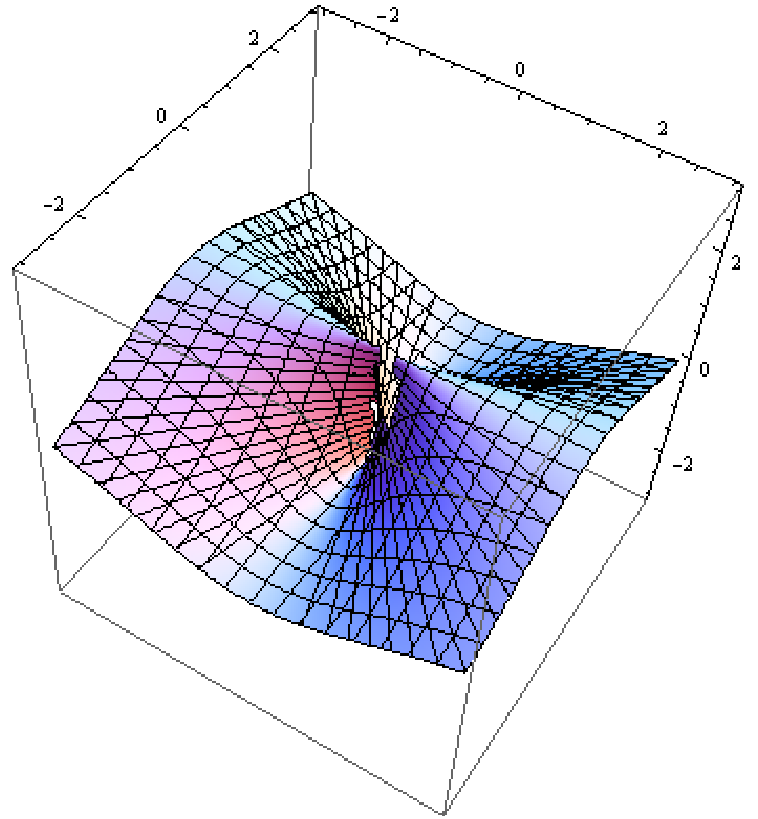
\includegraphics{./images/ch10/noLimEx.pdf}}
	\quad
	\resizebox{!}{4cm}{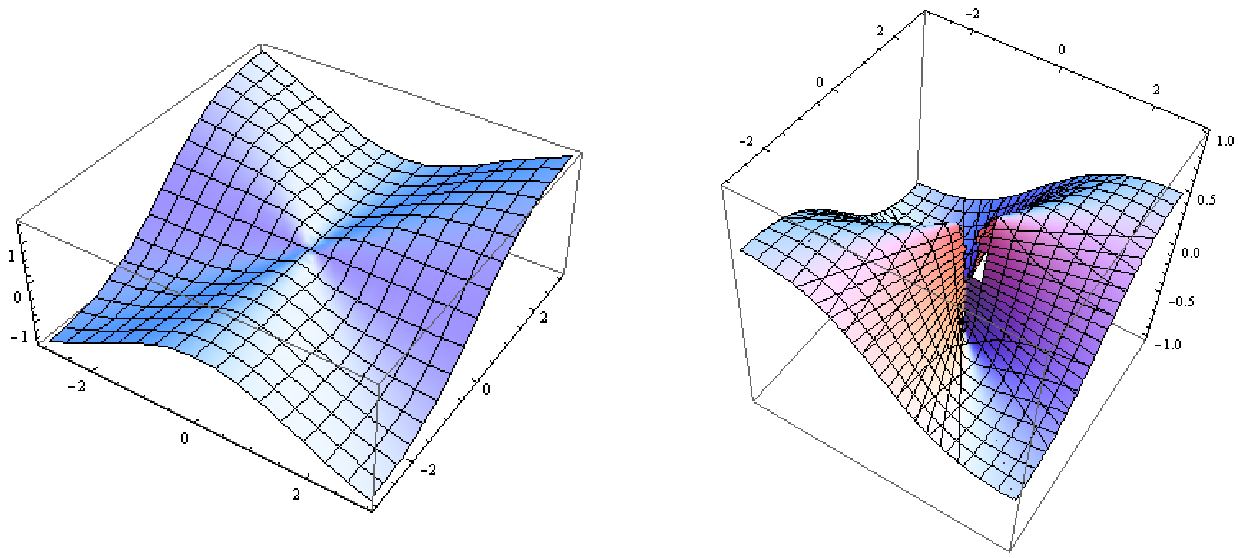
\includegraphics{./images/ch10/limEx.pdf}}
	
	教材-图10.1.13\hspace{2cm} 教材-图10.1.14\hspace{2cm} 教材-图10.1.15
\end{center}

{\bf 教材-例5:}证明极限$\lim\limits_{(x,y)\to(0,0)}\df{xy}{x^2+y^2}$不存在

{\bf 套路2:}若极限
$$\lim\limits_{{x\to x_0}\atop{y=y_0+k(x-x_0)}}f(x,y)$$
与$k$有关,则二重极限不存在。

套路2中的极限相当于从$(x,y)$出发,沿着直线趋于$(x_0,y_0)$。

无论套路1还是套路2,其中所涉及的都只是各种可能的趋近路线中的一部分,并能代表全面的情况,
因此,这两种套路只能用于证明二重极限不存在。

{\bf 教材-例4:}$\lim\limits_{(x,y)\to(0,0)}\df{x^2y}{x^2+y^2}$

{\bf 套路3:}令$x=x_0+\rho\cos\theta,y=y_0+\rho\sin\theta$,则
$$(x,y)\to(x_0,y_0)\quad\Leftrightarrow\quad\rho\to0$$
此时若极限
$$\lim\limits_{\rho\to{0^+}}f(\rho\cos\theta,\rho\sin\theta)$$
{\it 一致收敛},则对应二重极限存在。

{\bf 注:}
\begin{enumerate}[(1)]
  \setlength{\itemindent}{1cm}
  \item 所谓前述极限一致收敛,是指:存在常数$A$,对任意$\e>0$,存在
  $\delta>0$\ps{$\delta$的取值与$\theta$无关},
  对任意$\rho\in(0,\delta)$,恒有$|f(\rho\cos\theta,\rho\sin\theta)-A|<\e$
  \item 讨论前述极限时,不能简单地将$\theta$视为常数(相当于令$y=y_0+k(x-x_0)$),
  而是要求即使$\theta$为任意与$\rho$相关的函数,亦可保证极限的收敛
\end{enumerate}

{\bf 例:}证明:$\lim\limits_{(x,y)\to(0,0)}\df{x^2y^2}{x^2+y^2}=0$
	
[证]:令$\rho=\sqrt{x^2+y^2}$,$\tan\theta=\df yx$,则	
$$\lim\limits_{(x,y)\to(0,0)}\df{x^2y^2}{x^2+y^2}
=\lim\limits_{\rho\to{0^+}}\rho^2\cos^2\theta\sin^2\theta$$
对任意$\e>0$,令$\delta=\sqrt{\e}$,则对任意$\rho\in(0,\delta)$,总有
$$|\rho^2\cos^2\theta\sin^2\theta|<\e,$$
从而可知原二重极限存在,且为$0$。

{\bf 辅导书(下)-P12-例6-6:}讨论极限
$$\lim\limits_{(x,y)\to(0,0)}\df{xy^2}{x^2+y^4}$$
的存在性。

[证]:令$x=\rho\cos\theta,y=\rho\sin\theta$,则
$$\lim\limits_{(x,y)\to(0,0)}\df{xy^2}{x^2+y^4}
=\lim\limits_{\rho\to0^+}\df{\rho\cos\theta\sin^2\theta}
{\cos^2\theta+\rho^2\sin^4\theta}$$
我们可以证明,右端的极限不是一致收敛的。

显然,$\cos\theta=0$时,右端极限为$0$。

设$\cos\theta\ne 0$,则
$$\lim\limits_{\rho\to0^+}\df{\rho\cos\theta\sin^2\theta}
{\cos^2\theta+\rho^2\sin^4\theta}
=\lim\limits_{\rho\to0^+}\df{\rho\sin^2\theta}{\cos\theta},$$
对任意$k\in\mathbb{R},$若$\rho$和$\theta$满足
$\df{\rho\sin^2\theta}{\cos\theta}=k$,也即
$\rho^2\sin^2\theta=k\rho\cos\theta$,也即$ky^2=x$时,
则有
$$\lim\limits_{\rho\to0^+}\df{\rho\sin^2\theta}{\cos\theta}=k,$$
极限值与$k$有关,由此可见,原二重极限不存在。

% \begin{shaded}
% 	{\bf 二重极限与累次极限}
% 	
% 	{\bf 二重极限:}
% 	
% 	$$\lim\limits_{(x,y)\to(x_0,y_0)}f(x,y)$$
% 	
% 	{\bf 累次极限:}
% 	
% 	
% 	
% 	\begin{enumerate}[(1)]
%   	  \setlength{\itemindent}{1cm}
% 	  \item 若三者都存在,则值相等
% 	  \item 二重极限存在,累次极限必存在 
% 	  \item 两个累次极限均存在且相等,二重极限未必存在
% 	\end{enumerate}
% 	
% 	{\bf 思考:}如何从几何上解释三者之间的关系?
% 	
% 	\bigskip
% 	
% 	{\bf 关于用极坐标变换判定二重极限的存在性}
% 	
% 	讨论$\lim\limits_{(x,y)\to(x_0,y_0)}f(x,y)$
% 	的存在性时,可以令
% 	$$\rho=\sqrt{(x-x_0)^2+(y-y_0)^2},\quad \tan\theta=\df {y-y_0}{x-x_0},$$
% 	则
% 	$$(x,y)\to(x_0,y_0)\;\Leftrightarrow\;\rho\to0^+,$$
% 	从而
% 	$$\lim\limits_{(x,y)\to(x_0,y_0)}f(x,y)=\lim\limits_{\rho\to{0^+}}
% 	f(\rho\cos\theta,\rho\sin\theta).$$
% 	若右侧极限在$\rho\to{0^+}$的过程中与$\theta$的取值无关,则可以判定原极限存在。但
% 	要注意的是,这里不仅要求对任何固定的$\theta$(相当于沿着某条直线$y-y_0=k(x-x_0)$
% 	趋近$(x_0,y_0)$)	在$\rho\to{0^+}$时的极限与$\theta$无关,
% 	{\it 而且要求在$\rho\to{0^+}$过程中$\theta$可以随$\rho$的改变而取不同的值的情况
% 	下(例如沿着某条曲线$\rho=\rho(\theta)$趋近$(x_0,y_0)$)仍然无关,
% 	才能说明原极限存在。}
% 	
% 	{\bf 例:}证明:$\lim\limits_{(x,y)\to(0,0)}\df{xy}{x+y}$不存在
% 	
% 	{\bf 证:}令$\rho=\sqrt{x^2+y^2}$,$\tan\theta=\df yx$,则
% 	$$\lim\limits_{(x,y)\to(0,0)}\df{xy}{x+y}
% 	=\lim\limits_{\rho\to{0^+}}\df{\rho\cos\theta\sin\theta}
% 	{\cos\theta+\sin\theta}
% 	$$
% 	\begin{center}
% 		\resizebox{!}{6cm}{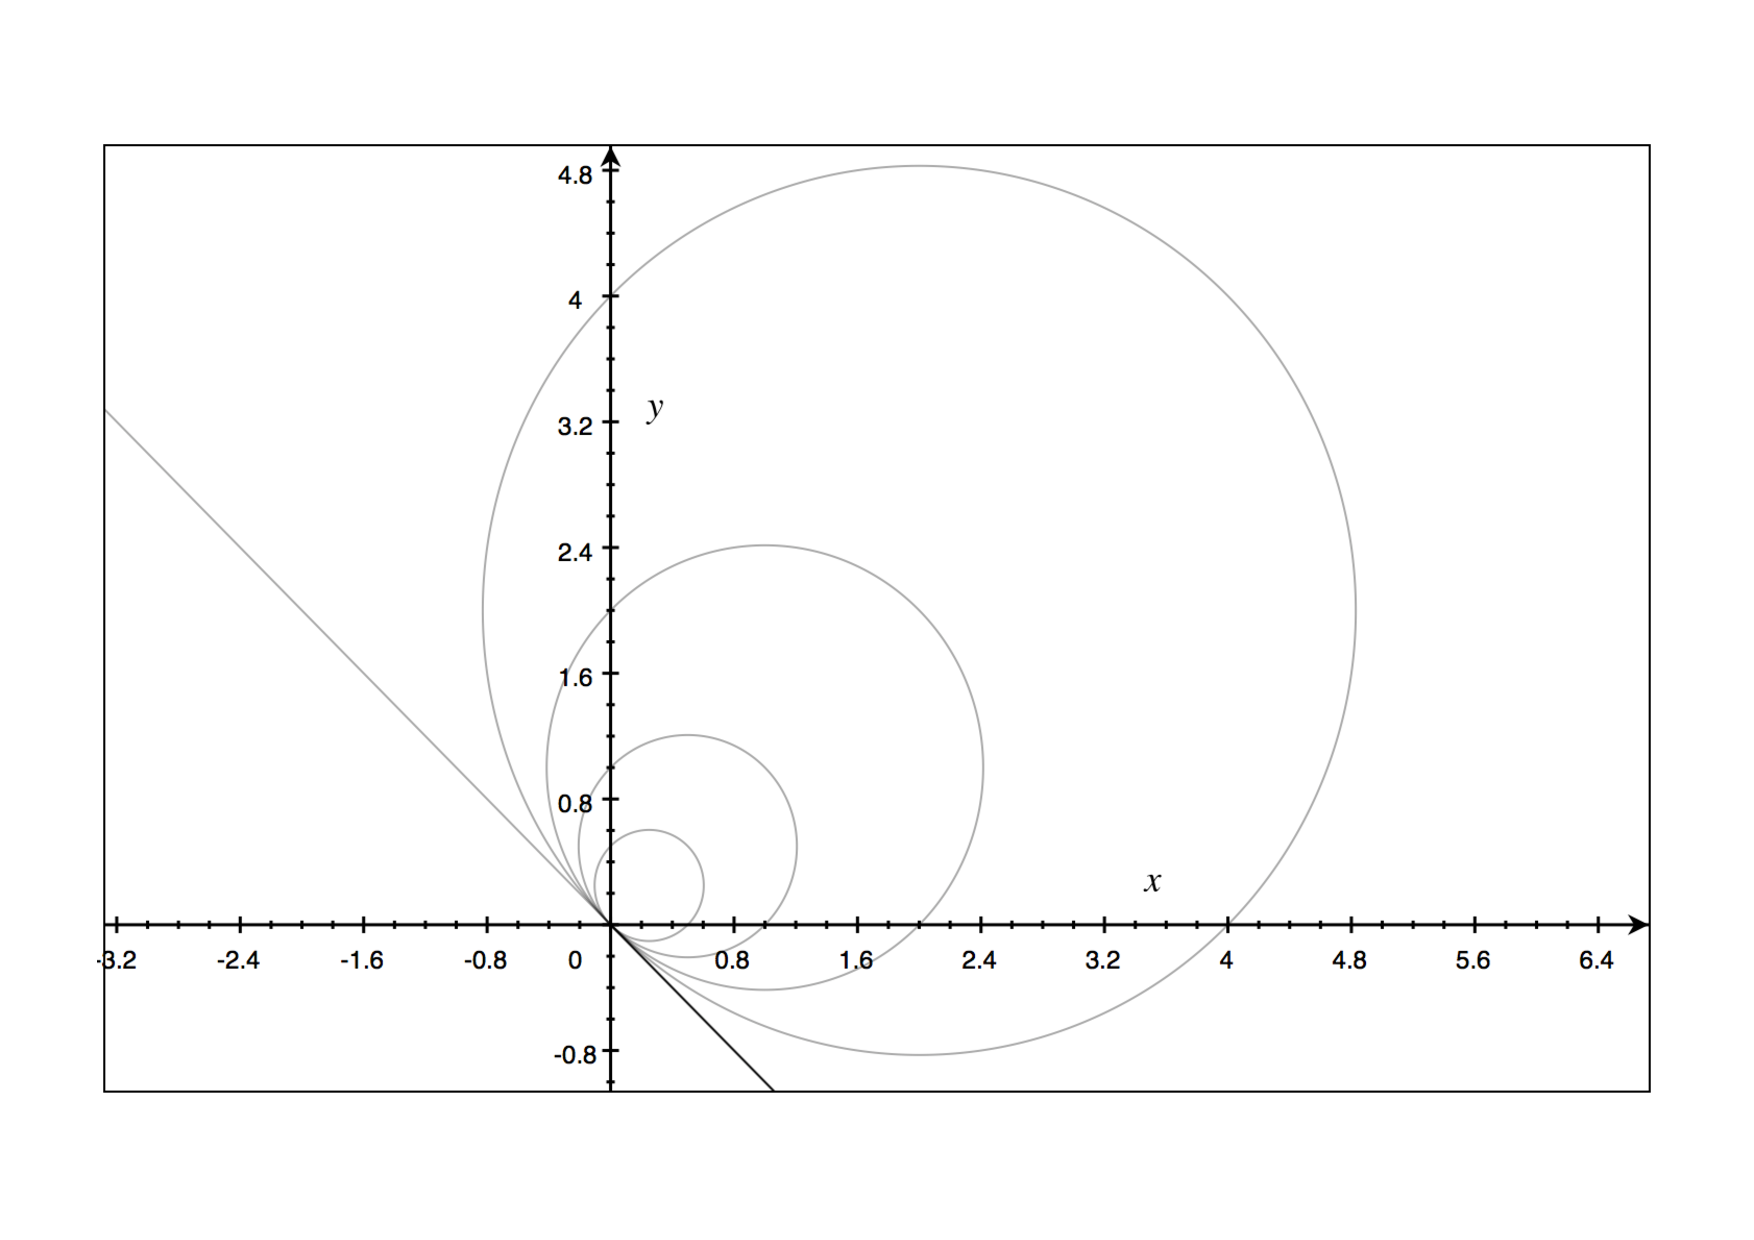
\includegraphics{./images/ch10/xy-xy.pdf}}
% 	\end{center}
% 	如图,考虑$(x,y)$沿$\rho=k(\cos\theta+\sin\theta)$趋于$(0,0)$,则
% 	当$\theta\to-\df{\pi}4$时,$\rho\to 0^+$,若原极限存在,则
% 	$$\lim\limits_{(x,y)\to(0,0)}\df{xy}{x+y}
% 	=\lim\limits_{\rho\to{0^+}}\df{\rho\cos\theta\sin\theta}
% 	{\cos\theta+\sin\theta}=\lim\limits_{\theta\to-\frac{\pi}4}
% 	k\cos\theta\sin\theta=-\df k2$$
% 	也即对应于不同的$k$值,极限计算的结果是不同的,故原极限不存在。
% 	
% 	{\bf 例:}证明:$\lim\limits_{(x,y)\to(0,0)}\df{x^2y^2}{x^2+y^2}=0$
% 	
% 	{\bf 证:}令$\rho=\sqrt{x^2+y^2}$,$\tan\theta=\df yx$,则	
% 	$$\lim\limits_{(x,y)\to(0,0)}\df{x^2y^2}{x^2+y^2}
% 	=\lim\limits_{\rho\to{0^+}}\rho^2\cos^2\theta\sin^2\theta$$	
% 	因为$\cos^2\theta\sin^2\theta\leq1$,故易知右侧极限与$\theta$无关且等于$0$,
% 	从而原极限等于$0$。
% 
% \end{shaded}

\subsection{多元函数的连续性}

{\bf $n$元函数$f(\bm{x})$在$\bm{x}_0$处连续:}

$$f(\bm{x}_0)=\lim\limits_{\bm{x}\to\bm{x}_0}f(\bm{x})$$

{\bf 注:}多元初等函数在其定义区间内连续

{\bf 例:}求函数$f(x,y)=\df{\arcsin(3-x^2-y^2)}{\sqrt{x-y^2}}$连续的区域。

\subsection{有界闭区域上连续函数的性质}

直接推广有界闭区间上连续的一元函数的性质,可得:

{\bf 定理:}设$D\in\mathbb{R}^2$为有界闭区域,$f(x,y)$在$D$上连续,则
\begin{enumerate}[(1)]
  \setlength{\itemindent}{1cm}
  \item $f(x,y)$必在$D$上有界
  \item $f(x,y)$必在$D$上取到最大$M$和最小值$m$
  \item 对于介于$M$和$m$之间的任意实数$c$,必存在$(\xi,\eta)\in{D}$,使得
  $f(\xi,\eta)=c$
\end{enumerate}

\section{偏导数与全微分}

\subsection{偏导数}

{\bf 二元函数$z=f(x,y)$在$(x_0,y_0)$处关于$x$的偏导数:}

\begin{eqnarray*}
	{f'_x(x_0,y_0)}  & = &
	\left.\df{\d}{\d x}f(x,y_0)\right|_{x=x_0} \\ 
	& = & \lim\limits_{x\to x_0}\df{f(x,y_0)-f(x_0,y_0)}{x-x_0} \\
	& = & {\left.\df{\p z}{\p x}\right|_{x=x_0,y=y_0}}
\end{eqnarray*}

{\bf 注:}偏导数等价于将其他变量视为常数所求得的导数

{\bf 例:}已知$f(x,y)=x^2+2xy$,求$f'_x(-1,1)$和$f'_y(-1,1)$。

{\bf $f'_x(x_0,y_0)$的几何意义:}空间曲线
$$\left\{\begin{array}{l}
z=f(x,y)\\ y=y_0
\end{array}\right.$$
在点$(x_0,y_0,f(x_0,y_0))$处的切线关于$x$轴的斜率

{\bf 教材-例2:}$f(x,y)=\left\{\begin{array}{cc}
	\df{xy}{x^2+y^2}, & (x,y)\ne (0,0)\\
	0, & else
\end{array}\right.$
求$f'_x(0,0)$和$f'_y(0,0)$

{\bf 注:}多元函数在一点偏导数存在,未必在该点连续!

\subsection{偏导数的计算}

运算规则:对指定变量求导时,将其他变量视为常数!

{\bf 例:}求以下函数的各个偏导数
\begin{enumerate}[(1)]
  \setlength{\itemindent}{1cm}
  \item $z=x^y$
  \item 已知$r=\sqrt{x^2+y^2+z^2}$,证明
	$$\left(\df{\p r}{\p x}\right)^2+\left(\df{\p r}{\p y}\right)^2+\left(\df{\p
	r}{\p z}\right)^2=1$$
\end{enumerate}

\subsection{高阶偏导数}

{\bf 二阶偏导数:}偏导数的偏导数 
$${f''_{xx}(x,y)=\df{\p}{\p x}\left(\df{\p z}{\p x}\right)
=\df{\p^2 z}{\p x^2}}$$ 
$${f''_{xy}(x,y)=\df{\p}{\p y}\left(\df{\p z}{\p x}\right)
=\df{\p^2 z}{\p x\p y}}$$ 
$${f''_{yy}(x,y)=\df{\p}{\p y}\left(\df{\p z}{\p y}\right)
=\df{\p^2 z}{\p y^2}}$$ 
$${f''_{yx}(x,y)=\df{\p}{\p x}\left(\df{\p z}{\p y}\right)
=\df{\p^2 z}{\p y\p x}}$$

{\bf 教材-例9:}验证函数$u=\sin(x-at)$满足{\bf 波动方程}
$\df{\p^2u}{\p t^2}=a^2\df{\p^2u}{\p x^2}$

{\bf 定理10.2.1:}若函数$z=f(x,y)$的两个混合偏导函数$f''_{xy}(x,y)$和$f''_{yx}(x,y)$
均在$(x_0,y_0)$处连续,则
$$f''_{xy}(x_0,y_0)=f''_{yx}(x_0,y_0)$$

\begin{itemize}
  \item 定理结论可推广到高阶偏导数的情形
  \item 求初等函数的高阶偏导数可任意选择求导顺序
\end{itemize}

\subsection{全微分}

\subsubsection{【二元函数的局部线性化】}

\begin{shaded}
	{\bf 一元函数$f(x)$在$x_0$处的微分}
	
	\begin{enumerate}[(1)]
  	  \setlength{\itemindent}{1cm}
	  \item {\bf 可微:}存在常数$A$,使得
	  $f(x)-f(x_0)=A\Delta x+\circ(\Delta x)$
	  \item {\bf 以直代曲:}用$x_0$处的切线近似替代$x_0$附近的函数值 
	  \item {\bf 微分:}$\d f(x)|_{x=x_0}=A\d x=f'(x_0)\d x$
	\end{enumerate}
\end{shaded}

{\bf 问题:}对于二元(或者多元)函数, 
\begin{itemize}
  \item 在什么情况下,存在类似的近似?
  \item 如何表达这样的近似? 
  \item 这种近似蕴含了哪些性质?
\end{itemize}

{\bf Insight:}切平面是平面上切线概念在高维空间中的推广:
用切平面近似替代$(x_0,y_0)$附近的函数值

{\bf 教材-例11:}求椭圆抛物面$S:z=2x^2+3y^2$在点$P(1,1,5)$处的切平面方程。

\begin{center}
	\resizebox{!}{4.7cm}{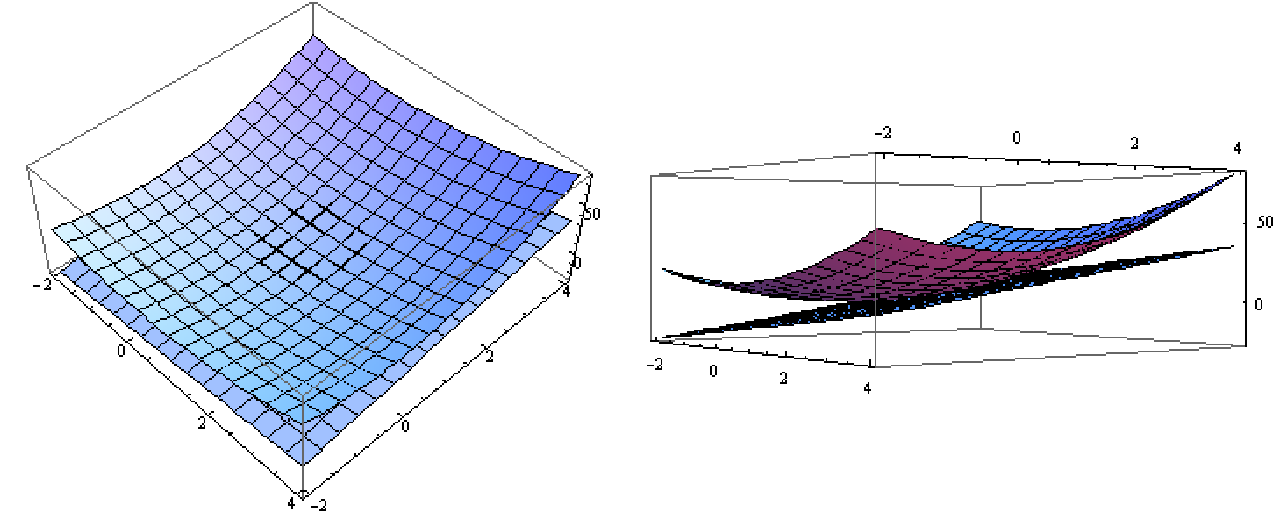
\includegraphics{./images/ch10/tangentFxy.pdf}}
	
	教材-图10.2.4:切平面:$z=4x+6y-5$或$z-5=4(x-1)+6(y-1)$
\end{center}

{\bf 教材-例12:}讨论函数$f(x,y)=\left\{\begin{array}{cc}
	\df{xy}{x^2+y^2},& (x,y)\ne (0,0)\\
	0, & else
\end{array}\right.$
在原点处的切平面。

\begin{center}
	\resizebox{!}{4.5cm}{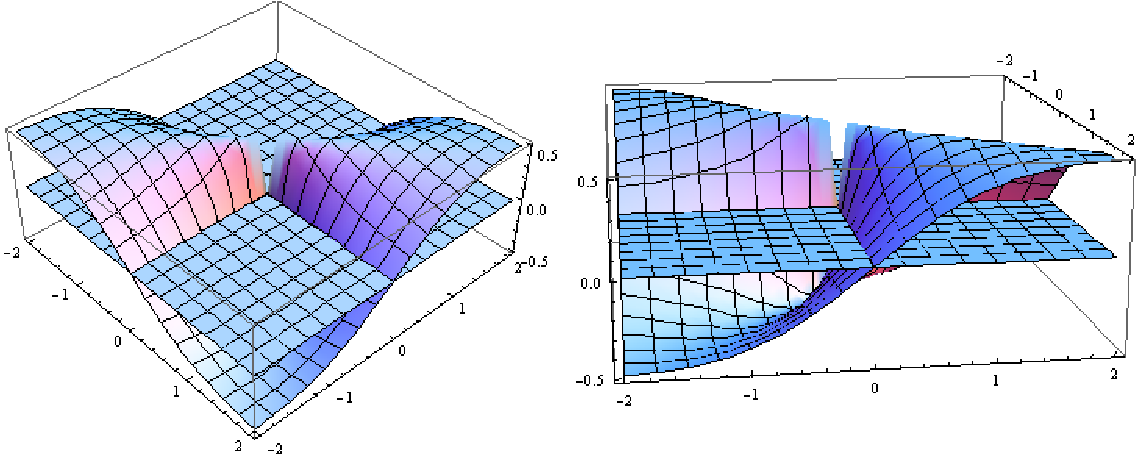
\includegraphics{./images/ch10/tangentNFxy.pdf}}
	
	参见教材-图10.1.14
\end{center}

{\bf 切平面:}两条特定方向的切线所张成的平面:

$$z\approx f(x_0,y_0)+f'_x(x_0,y_0)\Delta x+f'_y(x_0,y_0)\Delta y$$

\subsubsection{【(二元函数)全微分的概念】}

{\bf 定义:}设$z=f(x,y)$,
\begin{enumerate}[(1)]
  \setlength{\itemindent}{1cm}
  \item {\bf 可微:}存在常数$A,B$,使得
  $${\Delta z-A\Delta x-B\Delta y=\circ(\sqrt{\Delta x^2+\Delta y^2})}$$
  \item {\bf 以直代曲:}用$(x_0,y_0)$处的切平面近似替代附近的函数值
  \item {\bf 全微分:}$${\d z|_{(x_0,y_0)}=A\Delta x+B\Delta y}$$
\end{enumerate}

{\bf 例:}验证$z=2x^2+3y^2$在$(1,1,5)$处可微。

{\bf 注:}多元函数的全微分可以类似地加以定义。

\subsubsection{【全微分的性质】}

{\bf 定理10.2.1:}若二元函数$z=f(x,y)$在某点可微,则必在该点连续。

{\bf 例:}函数$f(x,y)=\left\{\begin{array}{cc}
	\df{xy}{x^2+y^2},& (x,y)\ne (0,0)\\
	0, & else
\end{array}\right.$
在原点处不连续,故不可微。

{\bf 定理10.2.2:}若二元函数$z=f(x,y)$在某点可微,则在该点处的偏导数
$\df{\p z}{\p x}$和$\df{\p z}{\p y}$均存在,且
$$\d z=\df{\p z}{\p x}\Delta x+\df{\p z}{\p y}\Delta y$$

\begin{itemize}
  \item 一般直接写做:
  $${\d z=\df{\p z}{\p x}\d x+\df{\p z}{\p y}\d y}$$ 
  \item 偏导数存在,函数不一定可微!
\end{itemize}

{\bf 教材-例15:}求$u=e^{x-y}+\sin z$在$(2,1,0)$处的全微分。

{\bf 定理10.2.3:}若二元函数$z=f(x,y)$在某点处的偏导函数
$\df{\p z}{\p x}$和$\df{\p z}{\p y}$连续,则$f(x,y)$在该点可微。

{\bf 注:}以上所有关于二元函数的结论都可以直接推广到$n$元函数的情形

\subsection*{小结}

\begin{enumerate}[(1)]
  \setlength{\itemindent}{1cm}
  \item {\bf 多元函数的极限与连续}
  \begin{itemize}
    \item 多重极限:沿任意路径逼近所得极限相同
    \item 累次极限存在且相等,多重极限未必存在
  \end{itemize}
  \item {\bf 偏导数}
  \begin{itemize}
    \item 对指定变量求导时,将其他变量视为常数
    \item 偏导存在,未必连续
    \item 几何意义:沿某坐标轴方向的切线斜率
  \end{itemize}
  \item {\bf 高阶偏导}
  \begin{itemize}
    \item 初等函数的高阶偏导与求导次序无关
  \end{itemize}
  \item {\bf 全微分}
  \begin{itemize}
    \item 何时可以对曲面进行“以直代曲”?\hfill 可微$\Leftarrow$偏导函数连续
    \item 对曲面“以直代曲”意味着什么?\hfill 曲面“光滑”$\Rightarrow$连续
    \item 全微分的基本形式:${\d z=\df{\p z}{\p x}\d x+\df{\p z}{\p y}\d y}$
    \hfill 全微分方程名称是怎么来的?
  \end{itemize}
\end{enumerate}

{\bf 思考:}为什么多元函数不能直接推广一元函数的导数定义呢?

\section{多元复合函数与隐函数的偏导数}

\subsection{多元复合函数求导}

{\bf 定理10.3.1}(多元函数求导的链式法则)
设$z=f(u,v),u=u(x,y),v=v(x,y)$, 且相关偏导数均存在, 则有
$${\df{\p z}{\p x}=\df{\p z}{\p u}\df{\p u}{\p x}
+\df{\p z}{\p v}\df{\p v}{\p x}}$$
$${\df{\p z}{\p y}=\df{\p z}{\p u}\df{\p u}{\p y}
+\df{\p z}{\p v}\df{\p v}{\p y}}$$

{\bf 注:}“嵌套”$\to$乘积,“并列”$\to$相加

{\bf 例:}对下列函数分别求$\df{\p z}{\p x}$和$\df{\p z}{\p y}$\hfill P127-128-例1,2
\begin{enumerate}[(1)]
  \setlength{\itemindent}{1cm}
  \item $z=e^u\cos v,u=2x-y,v=xy$
  \item $z=f(3x+2y,x^2+y^2)$
\end{enumerate}

\begin{shaded}
	{\bf 一些典型的情况}
	
	\begin{enumerate}[(1)]
  	  \setlength{\itemindent}{1cm}
	  \item $z=f(u,v),u=\varphi(x),v=\psi(x)$ 
	  \item $z=f(u,v,w),u=u(x,y),v=v(x,y),w=w(x,y)$ 
	  \item $z=f(u),u=\varphi(x,y)$ 
	  \item $z=f(x,u),u=\varphi(x,y)$
	\end{enumerate}
\end{shaded}

{\bf 教材-例3:}设$z=f(x,x+y,x/y)$,其中$f$可微,求$\df{\p z}{\p x}$
和$\df{\p z}{\p y}$

{\bf 教材-例4:}设$z=f(x/y)$,其中$f$可微,证明:$x\df{\p z}{\p x}+y
\df{\p z}{\p y}=0$

{\bf 教材-例5:}设$z=xy+xf(x/y)$,其中$f$可微,证明:
$$x\df{\p z}{\p x}+y\df{\p z}{\p y}=xy+z$$

{\bf 例:}设$z=uv+\sin t,u=e^t,v=\cos t$,求$\df{\d z}{\d t}$

{\bf 例:}设$z=f(xy,x^2-y^2)$,其中$f$具有二阶连续偏导函数,
求$\df{\p^2 z}{\p x^2}$和$\df{\p^2 z}{\p x\p y}$

\subsection{一阶微分的形式不变性}

{\bf 一元函数的微分形式不变性:}对于一元函数$f(x)$,无论$x$是自变量
还是中间变量,其一阶微分形式都是
$$\d y=f'(x)\d x$$

{\bf 多元函数的微分形式不变性:}$z=f(\varphi(x,y),\psi(x,y))$的全微分
$${\d z=\df{\p z}{\p x}dx+\df{\p z}{\p y}\d y
=\df{\p z}{\p u}\d u+\df{\p z}{\p v}\d v}$$
{\bf 无论$u,v$是自变量还是中间变量,其微分形式都一样}

{\bf 注:}利用一阶微分的形式不变性,可以通过求全微分的方法来求得一阶偏导数,但对于
高阶偏导数则不可以!

{\bf 多元函数全微分的运算法则:}
\begin{enumerate}[(1)]
  \setlength{\itemindent}{1cm}
  \item $\d(u\pm v)=\d u\pm \d v$
  \item $\d(cu)=c\d u\;(C\in\mathbb{R})$
  \item $\d(uv)=v\d u+u\d v$
  \item $\d\left(\df uv\right)=\df{u\d v-v\d u}{v^2}$
  \item $\d\left(\df 1v\right)=-\df{\d v}{v^2}$
\end{enumerate}

{\bf 教材-例8:}设$z=f(3x+2y,x^2+y^2)$,其中$f$可微,
求$\df{\p z}{\p x}$和$\df{\p z}{\p y}$

{\bf 例:}求$z=\arctan\df yx$的全微分和一阶偏导数。

{\bf 例:}设$z=f(x,x^2+y^2,x^2-y^2)$,其中$f$具有二阶连续偏导函数,
求$\df{\p^2 z}{\p x^2}$和$\df{\p^2 z}{\p x\p y}$

\subsection{隐函数的偏导数}

{\bf 隐函数:}蕴含在代数方程中的函数关系

{\bf 回顾:}对于包含两个变量的隐函数如何求导?

{\bf 思考:}对于形如
$$\left\{\begin{array}{l}
	  	x^2+y^2+z^2=4\\
	  	(x-1)^2+y^2=1
	  \end{array}\right.$$
的函数方程,该如何求(偏)导?

\subsubsection{【隐函数中的函数关系】}

\begin{enumerate}
  \setlength{\itemindent}{1cm}
  \item {\bf 一个方程所确定的隐函数} 
  $$F(x,y)=0 \quad \Rightarrow \quad y=f(x) $$
  $$F(x,y,z)=0 \quad \Rightarrow \quad z=f(x,y) $$
  \item {\bf 方程组所确定的隐函数} 
  $$\left.\begin{array}{l}
  	F(x,y,z)=0\\ G(x,y,z)=0
  \end{array}\right\} \quad \Rightarrow \quad 
  \left\{\begin{array}{l}
  	y=f(x)\\ z=g(x)
  \end{array}\right. $$
\end{enumerate}

{\bf Insight:}约束(方程)越多,自由度(自变量)越少!

{\bf 定理10.3.2}(隐函数存在定理)
若函数$F(x,y)$满足: 
\begin{enumerate}[(1)]
  \setlength{\itemindent}{1cm}
  \item $F(x_0,y_0)=0$ 
  \item $F(x,y)$在$(x_0,y_0)$附近偏导数连续 
  \item $F_y'(x_0,y_0)\ne 0$ 
\end{enumerate}
则:方程$F(x,y)=0$在$(x_0,y_0)$的某邻域内唯一确定一个函数$y=y(x)$,使得
在$x_0$附近满足$F(x,f(x))=0$, 且
$${\df{\d y}{\d x}=-\df{F'_x}{F'_y}}$$

{\bf 教材-例9:}设$2^{xy}=x+y$,求$\df{\d y}{\d x}$

{\bf 定理10.3.3}(隐函数存在定理)
若函数$F(x,y,z)$满足: 
\begin{enumerate}[(1)]
  \setlength{\itemindent}{1cm}
  \item $F(x_0,y_0,z_0)=0$ 
  \item $F(x,y,z)$在$(x_0,y_0,z_0)$附近偏导数连续 
  \item $F_z'(x_0,y_0,z_0)\ne 0$ 
\end{enumerate}
则:方程$F(x,y,z)=0$在$(x_0,y_0,z_0)$的某邻域内唯一确定一个函数$z=z(x,y)$,使得
在$(x_0,y_0)$附近满足$F(x,y,z(x,y))=0$, 且
$$\df{\p z}{\p x}=-\df{F'_x}{F'_z},\df{\p z}{\p y}=-\df{F'_y}{F'_z}$$

{\bf 教材-例10:}设$x^2+y^2+z^2=3xyz$,求$\df{\p z}{\p x},\df{\p z}{\p y}$

{\bf 教材-例11:}设$x^2y-e^z=z$,求$\df{\p z}{\p x},\df{\p z}{\p y}$
 和$\df{\p^2z}{\p x\p y}$
 
{\bf 教材-例13:}设$y=y(x),z=z(x)$由以下方程组确定,求$\df{\d y}{\d x},
 \df{\d z}{\d x}$

$$\left\{\begin{array}{l} x+y+z=0\\ x^2+y^2+z^2=1
\end{array}\right.$$

$$
	{\df{\d y}{\d x}=\df{\left|\begin{array}{cc}
		-1 & 1\\ -x & z
	\end{array}\right|}{\left|\begin{array}{cc}
		1 & 1\\ y & z
	\end{array}\right|}=\df{x-z}{z-y},} 
	{\df{\d z}{\d x}=\df{\left|\begin{array}{cc}
		1 & -1\\ y & -x
	\end{array}\right|}{\left|\begin{array}{cc}
		1 & 1\\ y & z
	\end{array}\right|}=\df{y-x}{z-y}}
$$

{\bf 教材-例14:}设$u=u(x,y),v=v(x,y)$由以下方程组确定,求$u'_x,u'_y$和$v'_x,v'_y$
$$
	\left\{\begin{array}{l}
		F(x,y,u,v)=0\\ G(x,y,u,v)=0
	\end{array}\right.
$$

{\bf 隐函数存在条件:}
\begin{enumerate}[(1)]
  \setlength{\itemindent}{1cm}
  \item $F,G$的所有一阶偏导连续
  \item {\bf Jacobi行列式:}
  $${J=\df{\p(F,G)}{\p(u,v)}=\left|\begin{array}{cc}
		F'_u & F'_v\\ G'_u & G'_v
	\end{array}\right|\ne 0}$$
\end{enumerate}

\subsubsection{【几何上的应用】}

{\bf 1、空间曲面的切平面和法线}

给定光滑曲面$S:F(x,y,z)=0$以及$P(x_0,y_0,z_0)\in S$

\begin{enumerate}[(1)]
  \setlength{\itemindent}{1cm}
  \item {\bf 过$P$的法向量:} ${(F'_x(P),F'_y(P),F'_z(P))}$ 
  \item {\bf 切平面:}
  	$$F'_x(P)(x-x_0)+F'_y(P)(y-y_0)+F'_z(P)(z-z_0)=0$$ 
  \item {\bf 法线:}
  	$$\df{x-x_0}{F'_x(P)}=\df{y-y_0}{F'_y(P)}=\df{z-z_0}{F'_z(P)}$$
\end{enumerate}

{\bf 推论:}若曲面方程为$z=f(x,y)$, 记
$$F(x,y,z)=f(x,y)-z,$$
则
$$F'_x=f'_x,\;F'_y=f'_y,\;F_z=-1,$$
若$f(x,y)$在$(x_0,y_0)$偏导数连续,则曲面在该点存在唯一的切平面和法线。

{\bf 2、空间曲线的切线和法平面}

给定曲线的一般式方程
$$\Gamma: \left\{\begin{array}{l}
	F(x,y,z)=0\\ G(x,y,z)=0
\end{array}\right.,$$
以及点$M\in\Gamma$

\begin{enumerate}[(1)]
  \setlength{\itemindent}{1cm}
  \item {\bf $P$处的切向量:} 
  $$\left(1,\left.\df 1J\df{\p(F,G)}{\p(z,x)}\right|_M,
  \left.\df 1J\df{\p(F,G)}{\p(x,y)}\right|_M\right)$$
  \item {\bf 法平面:}
  $$\left|
  		\begin{array}{ccc}
  			x-x_0 & y-y_0 & z-z_0\\
  			F'_x(M) & F'_y(M) & F'_z(M)\\
  			G'_x(M) & G'_y(M) & G'_z(M)
  		\end{array}
  	\right|=0$$
\end{enumerate}

{\bf 教材-例17:}求曲线$x^2+y^2+z^2=6,x+y+z=0$在点$M(1,-2,1)$处的切线和法平面方程。

$$\df{x-1}1=\df{y-1}{-1}=\df{z+2}0$$

$$x-y=0$$

\section{方向导数与梯度、Hessian矩阵及Taylor公式}

{\bf 回顾:}

设$z=f(x,y)$在$P(x_0,y_0)$可微,则$f\,'_x(x_0,y_0)$即为
\begin{itemize}
  \item 空间曲线
  $$C:\left\{\begin{array}{l}
  	z=f(x,y)\\ y=y_0
  \end{array}\right.$$
  在$(x_0,y_0,f(x_0,y_0))$的切线关于$x$的斜率
  \item {\it 曲面在$(x_0,y_0,f(x_0,y_0))$处沿$x$轴方向的切线斜率}
\end{itemize}

{\bf 问题:}能否/如何定义曲面在某点处沿任意方向的切线斜率?

\begin{enumerate}[(1)]
  \setlength{\itemindent}{1cm}
  \item 曲面$S:z=f(x,y)$ 
  \item $P(x_0,y_0,z_0)\in S$ 
  \item $xOy$平面内的二维向量$\bm{u}$ 
\end{enumerate}
求$z$在$P$处沿方向$\bm{u}$的变化率(斜率)。

\subsection{方向导数}

$z$在$P$处沿方向$\bm{u}$的变化率(斜率): 
$$k=\lim\limits_{h\to 0}\df{z(Q)-z(P)}{h}$$

{\bf $z=f(x,y)$在$(x_0,y_0)$沿$\bm{u}=(\cos\alpha,\cos\beta)$的方向导数:}

$${D_{\bm{u}}f(x_0,y_0)=\lim\limits_{h\to 0}
\df{f(x_0+h\cos\alpha,y_0+h\cos\beta)-f(x_0,y_0)}{h}}$$

{\bf 注:}$$D_{\bm{i}}f(x_0,y_0)=f\,'_x(x_0,y_0),
D_{\bm{j}}f(x_0,y_0)=f\,'_y(x_0,y_0)$$

{\bf 定理10.4.1:}
设函数$z=f(x,y)$在$P(x_0,y_0)$处可微, 则在该点处沿任意方向
$\bm{u}$的方向导数存在, 且
$$D_{\bm{u}}f(x_0,y_0) =f\,'_x(x_0,y_0)\cos\alpha+f\,'_y(x_0,y_0)\cos\beta$$
其中$\cos\alpha,\cos\beta$为$\bm{u}$的方向余弦。

{\bf 教材-例1:}求函数$f(x,y)=xe^{2y}+\cos(xy)$在点$(1,0)$处沿
$\bm{u}=(3,-4)$的方向导数。

{\bf 教材-例2:}求函数$f(x,y,z)=x^2\cos y+e^{-y}\ln(x+z)$在点$(1,0,0)$处沿
$\bm{u}=3\bm{i}-4\bm{j}$的方向导数。

\subsection{梯度(向量)}

{\bf 函数$z=f(x,y)$在$(x_0,y_0)$处的梯度:}

$$\bigtriangledown
f(x_0,y_0)=(f\,'_x(x_0,y_0),f\,'_y(x_0,y_0))=\bm{\mathrm{grad}}\,f$$

\begin{itemize}
  \item 梯度是一个向量
  \item 方向导数:梯度在所给定方向上的投影
  $${D_{\bm{u}}f(x_0,y_0)=\bigtriangledown f(x_0,y_0)\cdot\bm{e_u}}$$
  \item 梯度方向上的方向导数最大!
\end{itemize}

{\bf 教材-例4:}设某座山的表面对应于函数$z=15-3x^2-2y^2$,登山者站在其上的
$P(1,-2,4)$点,问其向哪个方向攀登坡度最陡?

\begin{itemize}
  \item 沿梯度方向攀登坡度最大 
  \item 梯度方向是函数值增加最快的方向 
\end{itemize}

{\bf 思考:}在画有等高线的地图上,如何判断何处最陡峭?

{\bf 梯度的几何意义:}$\bigtriangledown f$对应于$f(\bm{x})=c$的法线方向

\begin{center}
	\resizebox{!}{4.5cm}{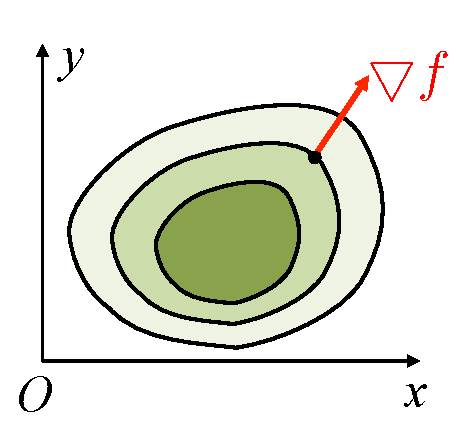
\includegraphics{./images/ch10/fxyc.pdf}}\hspace{3cm}
	\resizebox{!}{4.5cm}{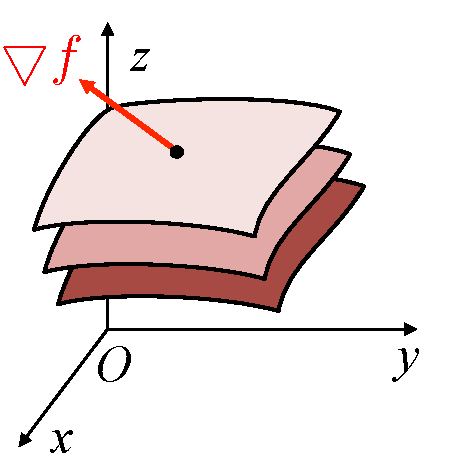
\includegraphics{./images/ch10/fxyzc.pdf}}
	
	等值(高)线:$f(x,y)=c$\hspace{3cm}等值面:$f(x,y,z)=c$
\end{center}

{\bf 【方向导数与梯度的应用】}

{\bf 定理10.4.2:}设$f(\bm{x})$在$\bm{x}_0$可微,$\bm{u}$为非零向量,
若$D_{\bm{u}}f(\bm{x}_0)>0$,则$\bm{u}$为
$f(\bm{x})$在$\bm{x}_0$处的一个上升方向;反之为一个下降方向。

{\bf 推论:}若$\bm{x}_0$为可微函数$f(\bm{x})$的一个{\it 局部最小(大)值}点,
则对任意$\bm{u}\ne 0$,$D_{\bm{u}}f(\bm{x}_0)=0$。

{\bf 注:}Fermat引理的推广!

\begin{shaded}
	{\bf 向量场与势函数}\dotfill{\it 以下文字摘自同济教材(下)P107}
	
	如果对于空间区域$G$内的任一点$M$,都有一个确定的数量$f(M)$与之对应,则称在
	该空间区域内确定了一个{\it 数量场}(例如:{\it 温度场、密度场}等)。一个数量
	场可用一个数量函数$f(M)$来确定。
	
	与之类似,如果与点$M$对应的是一个向量$\bm{F}(M)$,则称在该空间区域内确定了
	一个{\it 向量场}(例如:{\it 引力场、速度场})。一个向量场可用一个向量值函数
	$\bm{F}(M)$来确定。
	
	若向量场$\bm{F}(M)$是某个数量函数$f(M)$的梯度(也即$\bigtriangledown
	f=\bm{F}$),则称$f(M)$是向量场$\bm{F}(M)$ 的一个{\it 势函数},称$\bm{F}(M)$为{\it
	势场}。由此可知,由数量函数$f(M)$ 产生的梯度场$\bigtriangledown f(M)$是一个势场。
	但需要注意,{\it 并非每个向量场都是势场。}
	
\end{shaded}

\subsection{Hessian矩阵}

设$f(\bm{x})\,(\bm{x}=(x_1,x_2,\ldots,x_n))$的所有二阶偏导数连续 
$$H=\left[\begin{array}{cccc}
	\df{\p^2 f}{\p x_1^2} & \df{\p^2 f}{\p x_1\p x_2} & \ldots & \df{\p^2
	f}{\p x_1\p x_n}\\[10pt]
	\df{\p^2 f}{\p x_2\p x_1} & \df{\p^2 f}{\p x_2^2} & \ldots & \df{\p^2
	f}{\p x_2\p x_n}\\[10pt]
	\ldots & \ldots & \ldots & \ldots\\[6pt]
	\df{\p^2 f}{\p x_n\p x_1} & \df{\p^2 f}{\p x_n\p x_2} & \ldots & \df{\p^2
	f}{\p x_n^2}
	\end{array}\right]
=\bigtriangledown^2 f(\bm{x})$$

{\bf 教材-例6:}计算$f(x,y)=x^4+xy+(1+y)^2$的Hessian矩阵。

{\bf 教材-例7-8:}设$\bm{a},\bm{b},\bm{x}\in\mathbb{R}^n,\bm{Q}
\in\mathbb{R}^{n\times n},\bm{Q}=\bm{Q}^T,c\in\mathbb{R}$,
求以下函数的梯度与Hessian矩阵:
\begin{enumerate}[(1)]
  \setlength{\itemindent}{1cm}
  \item $f(\bm{x})=\bm{b}\bm{x}^{T}+c$
  \item $g(\bm{x})=\df 12\bm{x}\bm{Q}\bm{x}^T+\bm{b}\bm{x}^{T}+c$
\end{enumerate}

\subsection{多元Taylor公式}

{\bf 定理10.4.4:}设$n$元函数$f(\bm{x})$在$\bm{x}_0$的某邻域内二阶偏导数连续, 
则:对该邻域内任意点$\bm{x}$, 存在$\theta\in(0,1)$, 使得
\begin{eqnarray*}
	f(\bm{x}) & = & f(\bm{x}_0)+\bigtriangledown f(\bm{x}_0)(\bm{x}-\bm{x}_0)^T\\
	& & + \df 12(\bm{x}-\bm{x}_0)\bigtriangledown^2
	f(\bm{x}_0+\theta(\bm{x}-\bm{x}_0))(\bm{x}-\bm{x}_0)^T
\end{eqnarray*} 
即:{\bf $f(\bm{x})$在$\bm{x}_0$处带Lagrange余项的Taylor公式}

{\bf $f(\bm{x})$在$\bm{x}_0$处带Peano余项的Taylor公式:}

\begin{eqnarray*}
	f(\bm{x}) & = & f(\bm{x}_0)+\bigtriangledown f(\bm{x}_0)(\bm{x}-\bm{x}_0)^T\\
	& & + \df 12(\bm{x}-\bm{x}_0)\bigtriangledown^2
	f(\bm{x}_0)(\bm{x}-\bm{x}_0)^T+\circ(|\bm{x}-\bm{x}_0|^2)
\end{eqnarray*}

{\bf 教材-例9:}求$f(x,y)=x^4+xy+(1+y)^2$在原点处带Peano余项的一阶及二阶Taylor公式。

$$f(x,y)=1+2y+(xy+y^2)+\circ(x^2+y^2)$$

\begin{shaded}
	{\bf 二元函数$f(x,y)$在$(x_0,y_0)$处带Lagrange余项的的$n$阶Taylor公式:}
	设$f(x,y)$在$(x_0,y_0)$附近存在$n+1$阶偏导数,则存在$\theta\in(0,1)$,使得
	\begin{align*}
		f(x+\Delta x,y+\Delta y)&=\sum\limits_{k=0}^n
		\df1{k!}\left(\Delta x\df{\p}{\p x}+\Delta y\df{\p}{\p y}\right)^kf(x_0,y_0)\\
		&+\df1{(n+1)!}\left(\Delta x\df{\p}{\p x}+\Delta y\df{\p}{\p y}\right)
		^{n+1}f(x_0+\theta\Delta x,y_0+\theta\Delta y)
	\end{align*}
	其中
	$$\left(\Delta x\df{\p}{\p x}+\Delta y\df{\p}{\p y}\right)^kf(x_0,y_0)
	=\sum\limits_{p=0}^k\mathrm{C}_k^p\Delta x^p\Delta y^{k-p}
	\left.\df{\p^kf}{\p x^p\p y^{k-p}}\right|_{(x_0,y_0)}$$
	
	若记$\bigtriangledown=\left(\df{\p}{\p x},\df{\p}{\p y}\right)$,
	$\bm{x}=(x,y),\Delta\bm{x}=(\Delta x,\Delta y)$,则以上公式也可以表示为
	$$f(\bm{x}+\Delta\bm{x})=\sum\limits_{k=0}^n
	\df1{k!}\left(\Delta\bm{x}
	\cdot\bigtriangledown\right)^kf(\bm{x}_0)+\df1{(n+1)!}
	\left(\Delta\bm{x}\cdot\bigtriangledown\right)^{n+1}f(
	\bm{x}+\theta\Delta\bm{x})$$
	这种记号显然更加有利于将Taylor公式推广到更多元的函数情形。
	
	{\bf 例:}函数$f(x,y)=\ln(1+x+y)$在$(0,0)$处带Lagrange余项的三阶Taylor公式
	
	[解]:
	$$f'_x(x,y)=f'_y(x,y)=\df1{1+x+y}$$
	$$f''_{xx}(x,y)=f''_{xy}(x,y)=f''_{yy}(x,y)=-\df1{(1+x+y)^2},$$
	$$\df{\p^3f}{\p x^p\p y^{3-p}}=\df{2!}{(1+x+y)^3},\;p=0,1,2,3,$$
	$$\df{\p^4f}{\p x^p\p y^{4-p}}=-\df{3!}{(1+x+y)^4},\;p=0,1,2,3,4,$$
	故
	$$\left(\Delta x\df{\p}{\p x}+\Delta y\df{\p}{\p y}\right)f(0,0)
	=\Delta xf'_x(0,0)+\Delta yf'_y(0,0)
	=\Delta x+\Delta y,$$
	\begin{align*}
		\left(\Delta x\df{\p}{\p x}+\Delta y\df{\p}{\p y}\right)^2f(0,0)
		&=\Delta x^2f''_{xx}(0,0)+2\Delta x\Delta yf''_{x,y}(0,0)
		+\Delta y^2f''_{yy}(0,0)\\
		&=-(\Delta x+\Delta y)^2,
	\end{align*}
	\begin{align*}
		\left(\Delta x\df{\p}{\p x}+\Delta y\df{\p}{\p y}\right)^3f(0,0)
		&=\Delta x^3f'''_{xxx}(0,0)+3\Delta x^2\Delta yf'''_{xxy}(0,0)
		+3\Delta x\Delta y^2f'''_{xyy}(0,0)+\Delta y^3f'''_{yyy}(0,0)\\
		&=2(\Delta x+\Delta y)^3
	\end{align*}
	综上,存在$\theta\in(0,1)$,使得
	$$\ln(1+x+y)=x+y-\df12(x+y)^2+\df13(x+y)^3-\df14\df{(x+y)^3}
	{(1+\theta x+\theta y)^4}$$
\end{shaded}

\section{多元函数的极值与条件极值}

{\bf 极值:}局部唯一的最值

{\bf 定义:}{\bf $n$元函数$f(\bm{x})$在$\bm{x}_0$处取最小值:}
$f(\bm{x}_0)$有定义,且对$\bm{x}_0$某去心邻域内的任意点
$\bm{x}$,恒有$f(\bm{x})>f(\bm{x}_0)$

\begin{center}
	\resizebox{!}{4cm}{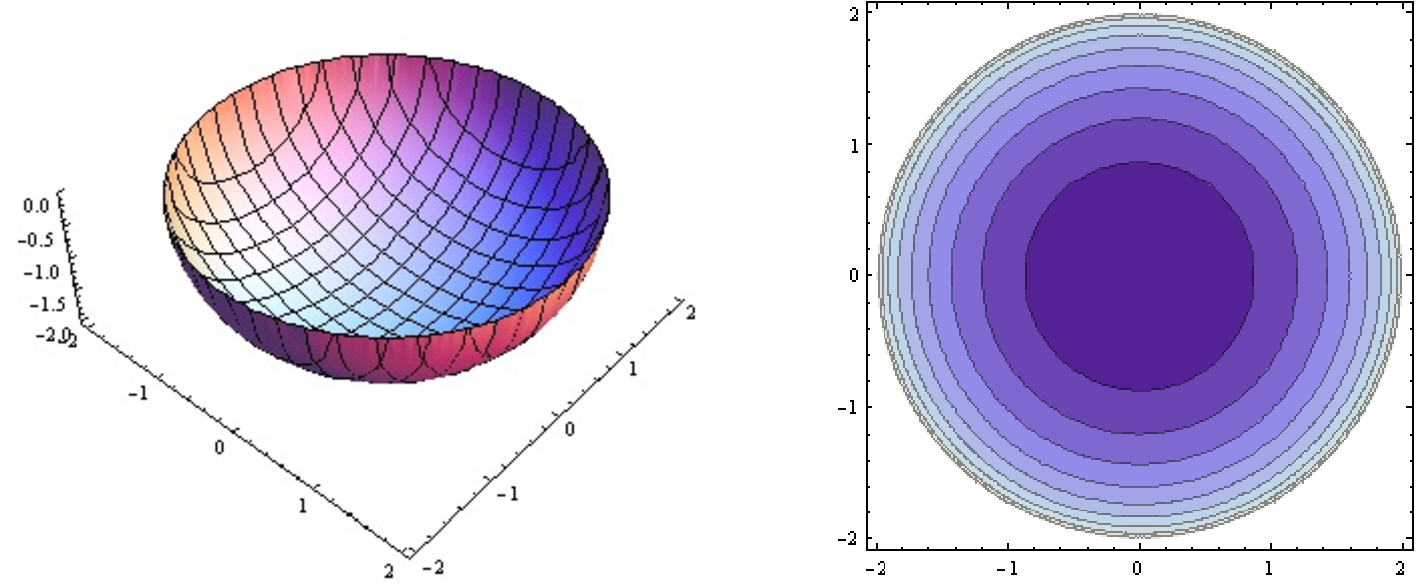
\includegraphics{./images/ch10/valley.pdf}}
	
	\resizebox{!}{4cm}{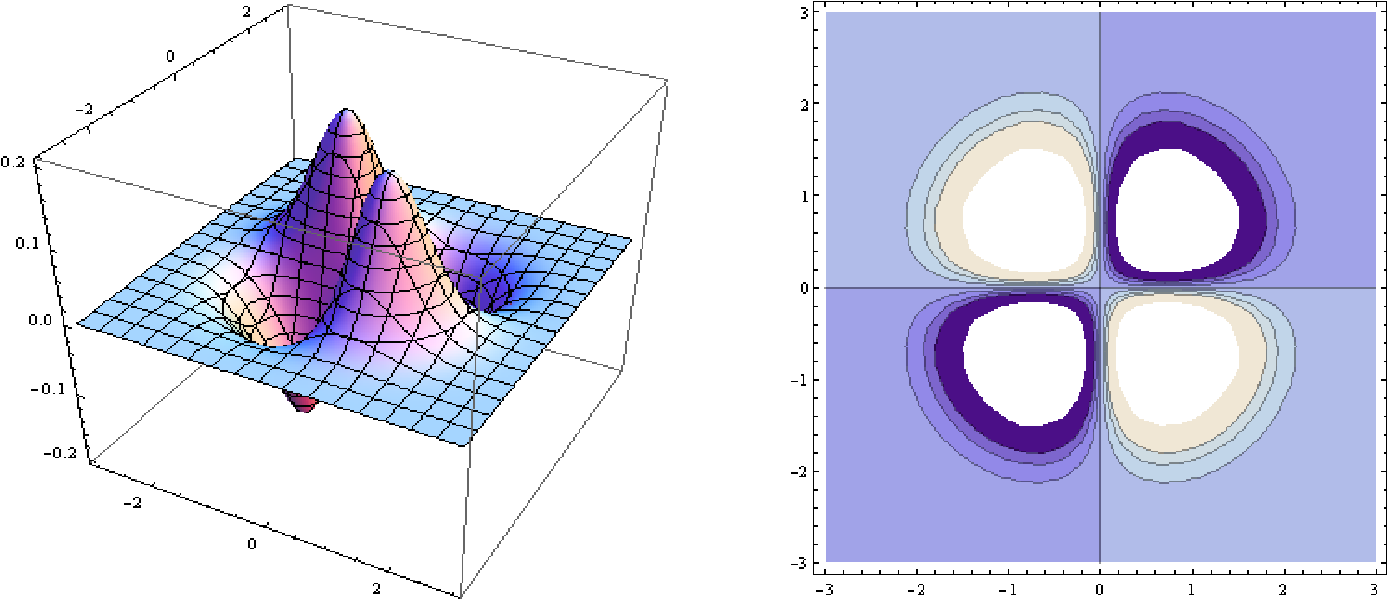
\includegraphics{./images/ch10/hill.pdf}}
\end{center}

\subsection{极值的判定}

\begin{itemize}
  \item {\bf 一元函数的极值点:}驻点、边界点或不可导点 
  \item {\bf 二元函数的极值点:}(二维)驻点、边界或“不可导”点 
\end{itemize}

\begin{center}
	\resizebox{!}{4cm}{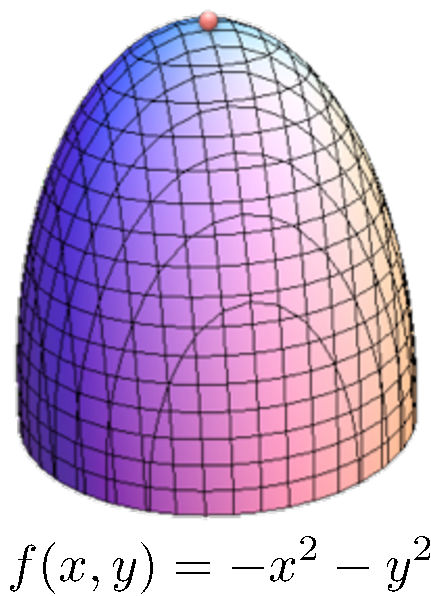
\includegraphics{./images/ch10/stayP.pdf}}\hspace{3cm}
	\resizebox{!}{4cm}{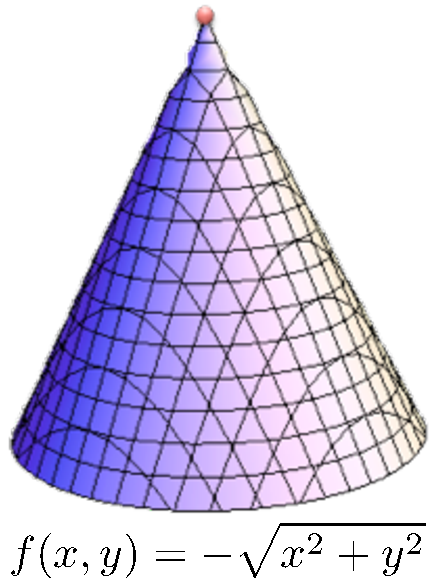
\includegraphics{./images/ch10/undevable.pdf}}
\end{center}

{\bf 定理10.5.1}(必要条件)若可微函数$f(\bm{x})$在$\bm{x}_0$处取极值,则$\bm{x}_0$
为$f(\bm{x})$的{\bf 驻点},即:$\bigtriangledown f(\bm{x}_0)=0$

{\bf 推论:}若$f(\bm{x})$在$\bm{x}_0$处偏导连续且取极值,则对应曲面
在该点处有水平切面。

\begin{shaded}
	{\bf 关于驻点:}
	
	\begin{itemize}
	  \item 可微函数的极值点必是驻点
	  \item 驻点未必是极值点 
	\end{itemize}
	
	\begin{center}
		\resizebox{!}{4cm}{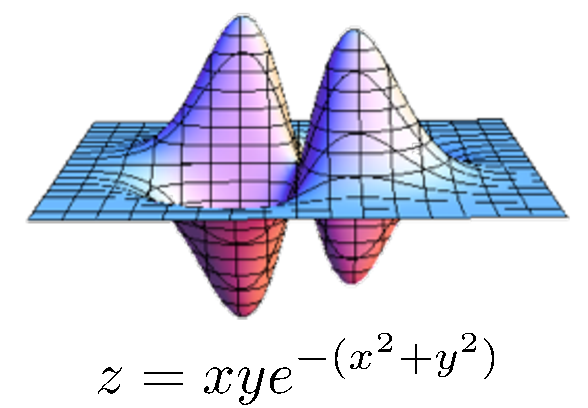
\includegraphics{./images/ch10/mhill.pdf}}\quad
		\resizebox{!}{4cm}{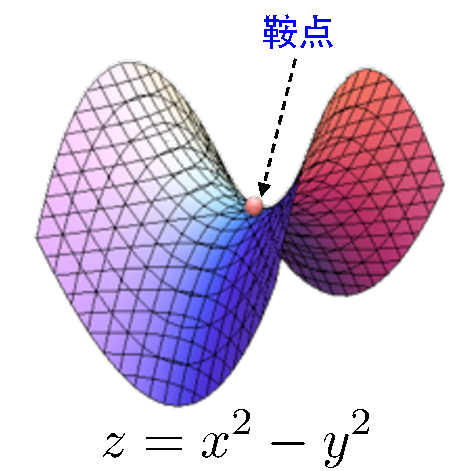
\includegraphics{./images/ch10/anhill.pdf}}
	\end{center}
\end{shaded}

{\bf 定理10.5.2}(充分条件)设$f(\bm{x})$在$\bm{x}_0$处存在二阶连续偏导数,
$\bigtriangledown f(\bm{x}_0)=0$,则由
$\bigtriangledown^2 f(\bm{x}_0)$正定、负定和不定
可分别判定$\bm{x}_0$为$f(\bm{x})$的极小值、极大值
和鞍点。

{\bf 注:}对多元函数而言,$\bigtriangledown f$和$\bigtriangledown^2 f$
类似于一元函数的一阶和二阶导数

{\bf 定理10.5.3}(二元函数极值的充分条件)

$f(x,y)$在$(x_0,y_0)$二阶偏导数连续,$\bigtriangledown f(x_0,y_0)=0$,
记$A=f\,''_{xx}(x_0,y_0),\,B=f\,''_{xy}(x_0,y_0),\,C=f\,''_{yy}(x_0,y_0)$,则
\begin{enumerate}[(1)]
  \setlength{\itemindent}{1cm}
  \item 若$A>0$且$AC-B^2>0$,$(x_0,y_0)$为$f(x,y)$的极小值点;
  \item 若$A<0$且$AC-B^2>0$,$(x_0,y_0)$为$f(x,y)$的极大值点;
  \item $AC-B^2<0$,$(x_0,y_0)$为$f(x,y)$的鞍点。
\end{enumerate}

{\bf 例:}求$z=-xye^{-(x^2+y^2)}$的极值。

\subsection{条件极值}

{\bf 教材-例4:}求函数$z=\sqrt{4-x^2-y^2}$的满足$(x-1)^2+y^2=1$的极值点。

\begin{center}
	\resizebox{!}{4cm}{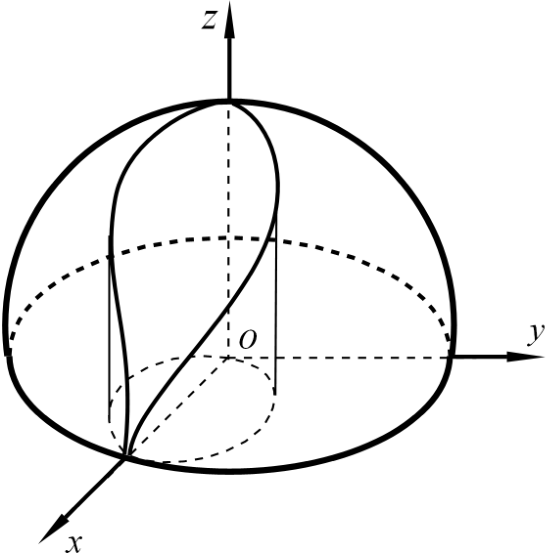
\includegraphics{./images/ch10/viviani.pdf}} 
\end{center}

{\bf 条件极值问题:}求某个多元函数$z=f(\bm{x})$满足一定条件$g(\bm{x})=0$的极值

{\bf 问题:}求$f(x,y)$满足$g(x,y)=0$的极值

{\bf 几何意义:}

\begin{center}
	\resizebox{!}{4.5cm}{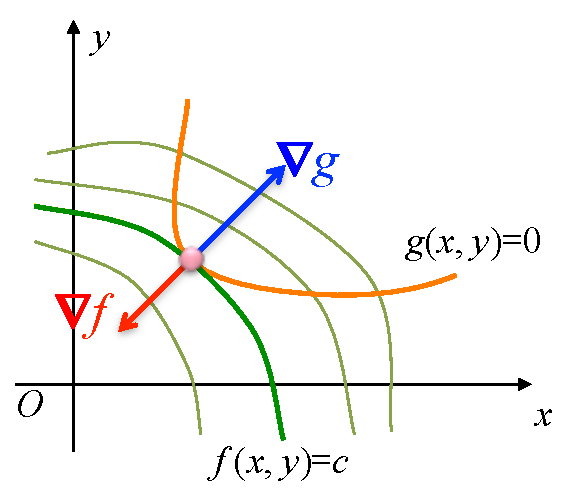
\includegraphics{./images/ch10/reshill.pdf}} 
\end{center}

若$f(x,y)=c$和$g(x,y)=0$光滑,则在极值点处必有
$${\bigtriangledown f // \bigtriangledown g}$$
即存在$\lambda_0$,使得
$$
{\left\{\begin{array}{l}
	f\,'_x(x_0,y_0)=\lambda_0g\,'_x(x_0,y_0)\\
	f\,'_y(x_0,y_0)=\lambda_0g\,'_y(x_0,y_0)
\end{array}
\right.}$$

{\bf 【Lagrange乘子法】}

{\bf Lagrange辅助函数:}
$${L(x,y,\lambda)=f(x,y)+\lambda g(x,y)}$$

\begin{enumerate}[(1)]
  \setlength{\itemindent}{1cm}
  \item $L(x,y,\lambda)$拥有相同的极值点 
  \item $L(x,y,\lambda)$的极值点$(x_0,y_0,\lambda_0)$满足 
  $$\bigtriangledown L(x_0,y_0,\lambda_0)=0$$
\end{enumerate}

{\bf 注:}Lagrange乘子法使我们能够在不必过度关注约束条件结构的情况下求解
条件极值问题。

{\bf 教材-例4:}求函数$z=\sqrt{4-x^2-y^2}$的满足$(x-1)^2+y^2=1$的极值点。

\begin{center}
	\resizebox{!}{6cm}{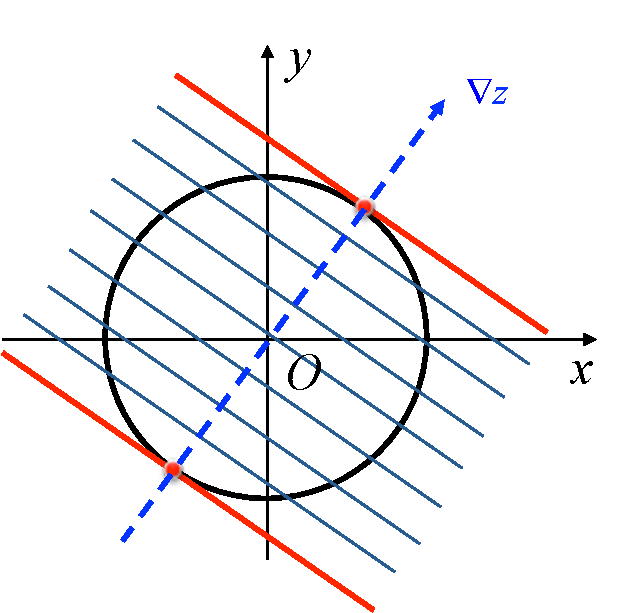
\includegraphics{./images/ch10/lagxy.pdf}}
\end{center}

{\bf 更一般情形的Lagrange乘子法:}

\begin{enumerate}[(1)]
  \setlength{\itemindent}{1cm}
  \item {\bf 更高维:} 函数$w=f(x,y,z)$满足$g(x,y,z)=0$的极值 
  
  [解]:记$L=f(x,y,z)+\lambda g(x,y,z)$,令$\bigtriangledown L=0$ 
  \item {\bf 更多约束:} 函数$w=f(x,y,z)$满足$g_1(x,y,z)=g_2(x,y,z)=0$的极值 
  
  [解]: 记
  $$L=f(x,y,z)+\lambda_1 g_1(x,y,z)+\lambda_2 g_2(x,y,z),$$
  令$\bigtriangledown L=0$
\end{enumerate}

{\bf 教材-例7:}求平面$x+y+z=1$与柱面$x^2+y^2=1$上距离原点最近和最远的点。

\begin{center}
	\resizebox{!}{5cm}{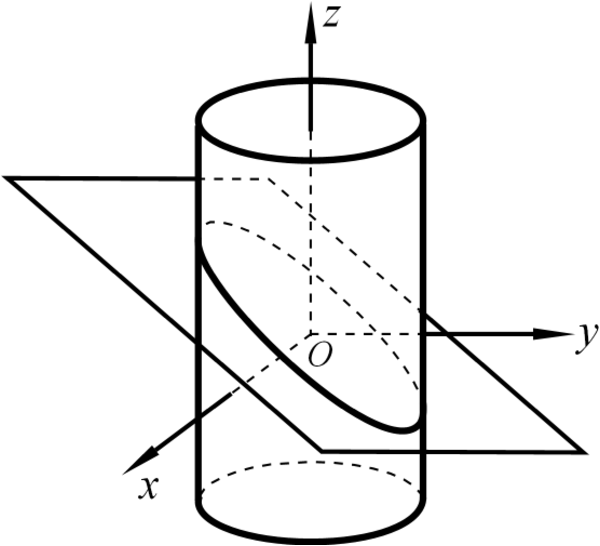
\includegraphics{./images/ch10/planeCy.pdf}}
\end{center}

{\bf 教材-例6:}要制作一个表面积为$a^2$的无盖长方体盒子,
问其长宽高各为多少时,盒子的容积最大。

$$x=y=\df a{\sqrt 3},\;z=\df a{2\sqrt3}$$
$$V_{\max}=\df{a^2}{6\sqrt 3}$$

\section{小结}

多元函数微分学是对一元函数微分学的推广,通过本章的学习,应该会对此留下比较深刻的印象。

然而,与从一元函数推广到向量值函数时的那种“轻松自如”不同,从一元到多元的推广显然要
复杂得多。在本章的学习中要特别注意把握两者的异同。

不同的地方,主要源自两个方面,一是从一维集合上升到二维集合,导致极限概念在理解上的差异
(从数学形式上看没有什么不同),二是从导数概念简单形式推广中遇到的问题(向量不能作分母),
导致在可导、可微概念上出现了诸多的差异。可以说,从一元微分学到多元微分学,一直是有异
有同相互交织的,能够在相互比照,理解推广的原理的同时,准确把握前后的差异,是深刻理解
本章所有结论的根本。

\begin{enumerate}
  \item {\bf 极限与连续}
  \begin{enumerate}[(1)]
    \item 二重极限存在性的判定
    \begin{itemize}
      \item {\it 套路1}:累次极限不同,则二重极限不存在
      \item {\it 套路2}:令$y=kx$,若相应的极限与$k$有关,则二重极限不存在
      \ps{\b 与$k$无关并不能说明二重极限存在!}
      \item {\it 套路3}:令$x=\rho\cos\theta,y=\rho\sin\theta$,则
      $(x,y)\to(x_0,y_0)\Leftrightarrow\rho\to0^+$,若极限
      $$\lim\limits_{\rho\to0^+}f(\rho\cos\theta(\rho),\rho\sin\theta(\rho))$$
      为常数,则二重极限存在。\ps{\b $\theta(\rho)$表示$\theta$的取值可能是与$\rho$有关的!}
%       二重极限与累次极限的关系:
%       $\lim\limits_{(x,y)\to(x_0,y_0)}f(x,y)=a\Rightarrow
%       \lim\limits_{x\to x_0}\lim\limits_{y\to y_0}f(x,y)=
%       \lim\limits_{y\to y_0}\lim\limits_{x\to x_0}f(x,y)=a$,反之不然!
%       \item 判定二重极限不存在:选择不同的路径,证明相应的极限不存在,即:若
%       对过$(x_0,y_0)$不同的连续曲线$y=y(x,k)$(例如$y=kx$),
%       $$\lim\limits_{x\to x_0\atop y=y(x,k)}f(x,y)=a(k)$$
%       不为常数,则二重极限不存在
%       \item 判定二重极限存在:利用极坐标变换,将$(x,y)\to(x_0,y_0)$转换为$\rho\to0^+$,
%       证明极限
%       $$\lim\limits_{\rho\to0^+}f(\rho\cos\theta(\rho),\rho\sin\theta(\rho))$$
%       为常数。
      
%       注意:{\it $\theta(\rho)$表示$\theta$的取值可能是与$\rho$有关的!}
      \item 重点掌握教材10.2节的例3-例5
      \item 注意各种不同极限形式的正确书写方法,例如
      $$\lim\limits_{(x,y)\to(x_0,y_0)}f(x,y)\quad
      \lim\limits_{x\to x_0\atop y\to y_0}f(x,y),\quad
      \lim\limits_{x\to x_0}\lim\limits_{y\to y_0}f(x,y),\quad
      \lim\limits_{x\to x_0\atop y=kx}f(x,y),\quad
      \lim\limits_{x\to x_0\atop y=0}f(x,y)
      $$
    \end{itemize}
    \item 连续与可微
    \begin{itemize}
      \item 有界闭区域上的多元连续函数与有界闭区间上的一元连续函数具有类似的性质:
      有界性、最值存在性和介值性
      \item 可微必连续,且偏导数存在
      \item 用定义证明$z=f(x,y)$在$(x_0,y_0)$可微:令$A=f'_x(x_0,y_0),B=f'_y(x_0,y_0)$,
      证明
      $$\lim\limits_{(0,0)\to(x_0,y_0)}
      \df{f(x_0+\Delta x,y_0+\Delta y)-f(x_0,y_0)
      -A\Delta x-B\Delta
      y}{\sqrt{(\Delta x)^2+(\Delta y)^2}}=0$$
      即可
      \item 重点掌握教材习题10.2节的16-17.
    \end{itemize}
  \end{enumerate}
  \item {\bf 偏导数、全微分与方向导数}
  \begin{enumerate}[(1)]
    \item 偏导数及其计算
    \begin{itemize}
      \item 偏导数的定义:除求导变量外,将其他自变量均视为常数(因此在实际计算某个
      点处的偏导时,可以先带入其他自变量的值)然后求导,例如
      $$\left.\df{\p}{\p x}(1+x+\arctan(xy))\right|_{(2,0)}=
      \left.\df{\d}{\d x}(1+x)\right|_{x=2}=1$$
      \item 偏导数的几何意义:$f'_x(x_0,y_0)$表示曲线$\left\{\begin{array}{l}
      z=f(x,y)\\ y=y_0
      \end{array}\right.$在$(x_0,y_0)$处的切线斜率,也相当于在该点处沿$\bm{i}$方向
      的方向导数$D_if(x_0,y_0)$
      \item 复合函数的偏导数:设$z=f(u,v),u=u(x,y),v=v(x,y)$,则
      $$z'_x=z'_uu'_x+z'_vv'_x$$
      {\it 链式法则:}画出变量之间的依赖关系图(树),标记出每条路线上对应的偏导数,
      按照“并联对应加法,串联对应乘法”的规则,综合写出所有可能的路径
      \item 隐函数求导:(1)确定那些变量是自变量,那些是因变量;(2)对所有给定的方程
      两边求(偏)导,解出相应的(偏)导数值;或者(2')对所有方程求全微分,解出所有因变量
      的全微分,然后根据一阶微分的形式不变性,确定相应的(偏)导数
    \end{itemize}
    \item 全微分:设$z=f(x,y)$,则
    $$\d z=f'_x\d x+f'_y\d y=\bigtriangledown f\cdot \d\bm{r},$$
    其中$\d\bm{r}=(\d x,\d y)$
    \begin{itemize}
      \item 全微分的应用:误差估计、判断不同参数(的误差)对测量值(的误差)的影响
    \end{itemize}
    \item 方向导数与梯度
    \begin{itemize}
      \item 方向导数的定义(以二元函数为例)
      $$\left.\df{\p f}{\p u}\right|_{(x_0,y_0)}=D_uf(x_0,y_0)
      =\lim\limits_{h\to0}\df{f(x_0+h\cos\theta,y_0+h\sin\theta)-
      f(x_0,y_0)}{h}$$
      其中$\bm{u}=|\bm{u}|(\cos\theta,\sin\theta)$
      \item 若$z=f(x,y)$可微,则沿任意方向的方向导数存在,且
      $$D_uf=\bigtriangledown f\cdot\bm{e}_u=\left(\bigtriangledown f\right)_u$$
      \begin{itemize}
        \item 推论1:沿梯度方向的方向导数值最大
        \item 推论2:梯度方向是该点处的最快上升方向
        \item 推论3:梯度方向垂直与该点处的等高线,且指向函数值增大的方向,例:
        (1)球面的{\it 外法向}为指向球外部的矢径方向
        (2)曲面$F(x,y,z)=0$可视为函数$w=F(x,y,z)$的一个等值面,故其法向量为 
        $\bigtriangledown F$
      \end{itemize}
    \end{itemize}
  \end{enumerate}
  \item {\bf 多元函数微分学的应用}
  \begin{enumerate}[(1)]
    \item 注意:
    \begin{itemize}
      \item 与一元函数相关概念的对应关系:梯度$\bigtriangledown f\leftrightarrow$一阶导数$f'$,
      Hessian矩阵$\bigtriangledown^2f\leftrightarrow$二阶导数$f''$
      \item 与一元函数相关方法的异同 
    \end{itemize}
    \item Taylor公式(以二元函数为例):$z=f(x,y)$在$(x_0,y_0)$处带Peano余项的二阶Taylor公式
      \begin{eqnarray*}
      f(x,y)&=&f(x_0,y_0)+\bigtriangledown
      f(x_0,y_0)\left[\begin{array}{c}
      x-x_0\\ y-y_0
      \end{array}\right]\\
      &&+\df12(x-x_0\;y-y_0)\bigtriangledown^2f(x_0,y_0)
      \left[\begin{array}{c}
      x-x_0\\ y-y_0
      \end{array}\right]+\circ((x-x_0)^2+(y-y_0)^2)
	\end{eqnarray*}
	\begin{itemize}
	  \item $n$次多项式函数的$m$阶Taylor多项式就是其$m$次阶段多项式
	\end{itemize}
    \item 极值问题
    \begin{itemize}
      \item 可能的极值点:驻点($\bigtriangledown f=0$)、不可微点和边界点
      
      注意:边界部分的处理!例:$z=\sqrt{x^2+y^2}$在如下区域上的极值:(1)
      $|x|\leq1,|y|\leq1$;(2)$x^2+y^2\leq 1$;(3)$x^2+y^2\leq 1,x\geq 1$
      \item Fermat引理的推广:可微函数的极值点必为驻点!
      \item 可微函数的极值判定:若$\bigtriangledown f=0$,且$\bigtriangledown^2f$
      正(负)定,则取极小(大)值
    \end{itemize}
    \item 条件极值问题
    \begin{itemize}
      \item 对于经典极值问题的另一种叙述:任何极值问题都可以表述为一个目标函数和多个约束
      关系的组合,例如:求(目标函数)$z=f(x,y)$满足(约束关系)$g(x,y)=0$的极值
      \item 解法一:利用约束解出变量的对应关系,带回目标函数,求解极值问题
      \item 解法二:Lagrange乘子法
      \begin{itemize}
        \item 几何意义:$\bigtriangledown f//\bigtriangledown g$
        \item Lagrange函数
        $$L(x,y,\lambda)=f(x,y)+\lambda g(x,y)$$
        与目标函数有相同的极值!
        \item 解题要点:(1)合理确定变量,分清目标函数与约束条件;(2)极值类型的判定
      \end{itemize}
    \end{itemize}
  \end{enumerate}
\end{enumerate}

{\it 一些重要概念的相互关系:}

\begin{center}
	\resizebox{!}{4.5cm}{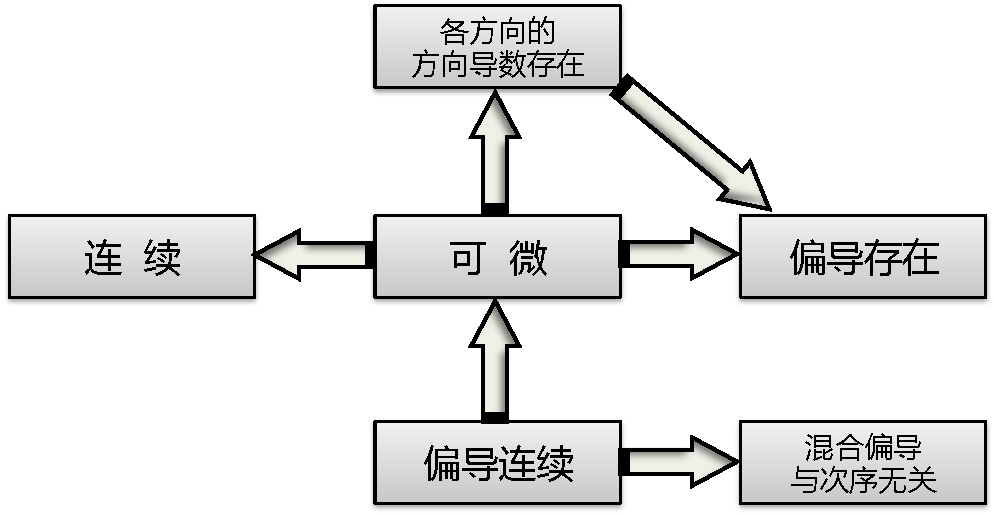
\includegraphics{./images/ch10/drela.pdf}} 
\end{center}

\begin{shaded}
{\bf 相关的反例}

1、连续但偏导不存在(连续但不可微)

$$f(x,y)=\sqrt{x^2+y^2}$$

2、偏导存在但不连续(偏导存在但不可微)

$$
f(x,y)=\left\{\begin{array}{ll}
0 & ,(x,y)=(0,0)\\
\df{xy}{x^2+y^2}& ,else
\end{array}\right.
$$

3、可微但偏导不连续

$$
f(x,y)=\left\{\begin{array}{ll}
0 & ,(x,y)=(0,0)\\
(x^2+y^2)\sin\df1{x^2+y^2}& ,else
\end{array}\right.
$$

4、偏导不连续且混合偏导数不相等

$$
f(x,y)=\left\{\begin{array}{ll}
0 & ,(x,y)=(0,0)\\
xy\df{x^2-y^2}{x^2+y^2}& ,else
\end{array}\right.
$$

5、连续、偏导存在且任意方向的方向导数(按同济教材的定义)均存在但不可微

$$
f(x,y)=\left\{\begin{array}{ll}
0 & ,(x,y)=(0,0)\\
\df{\sqrt{|xy|}}{x^2+y^2}\sin(x^2+y^2)& ,else
\end{array}\right.
$$

6、所有的方向导数(按KD教材的定义)存在而不可微

$$
f(x,y)=\left\{\begin{array}{ll}
0 & ,y=0\\
\df{x^2+y^2}{y}& ,else
\end{array}\right.
$$

7、方向导数(按同济教材的定义)满足$D_uf=f'_x\cos\theta+f'_y\sin\theta\;
(u=\rho\sin\theta)$但不可微,甚至不连续

$$
f(x,y)=\left\{\begin{array}{ll}
y=\rho\sin\theta & ,(x,y)\in D_1\\
1& ,(x,y)\in D_2\\
0& ,else
\end{array}\right.
$$
其中$D_1$为心形线$\rho=1-\cos\theta$及其内部,$D_2$表示其外部,且不在$x$轴上。

[提示]: $f'_x(0,0)=0,f'_y(0,0)=1,D_uf=\sin\theta$,在$D_2$
内总存在靠近$(0,0)$的某点,使得
$$|f(x,y)-f(0,0)-[f'_x(0,0)x+f'_y(0,0)y]|=1$$


\end{shaded}

\newpage

\section*{习题课}
\addcontentsline{toc}{section}{习题课}

\subsection*{多元函数的极限、连续、偏导数与全微分}

{\bf 辅导(下)-P12-例6-6:}讨论极限$\lim\limits_{(x,y)\to(0,0)}\df{xy^2}{x^2+y^4}$

$$\lim\limits_{x\to 0\atop{y=kx}}\df{xy^2}{x^2+y^4}=0$$

$$\lim\limits_{x\to 0\atop{y^2=x}}\df{xy^2}{x^2+y^4}=\df12$$

{\bf 辅导(下)-P12-例6-7:}证明极限$\lim\limits_{(x,y)\to(0,0)}(1+xy)
^{\frac1{x+y}}$不存在


$$\lim\limits_{x\to 0\atop{y=kx}}(1+xy)^{\frac1{x+y}}=1\quad (k\ne -1)$$

$$\lim\limits_{x\to 0\atop{y=x^2-x}}(1+xy)^{\frac1{x+y}}=e^{-1}$$

{\bf 辅导(下)-P12-例6-8:}证明极限$\lim\limits_{(x,y)\to(0,0)}
\df{x^3+xy^2}{x^2-xy+y^2}=0$

{\bf 例:}证明函数
  $$f(x,y)=\left\{\begin{array}{cc}
  	\df{x^2y}{x^2+y^2},& (x,y)\ne (0,0)\\
  	0,& else
  \end{array}\right.$$
  在原点可微,但偏导数不连续。

{\bf 辅导(下)-P16-例6-16:}证明:$z=\sqrt|xy|$在
原点连续,偏导数存在,但不可微。

{\bf 课后思考:}习题8.2:16-18

{\bf 辅导(下)-P17-例6-17:}正六棱台的上下底和高分别为$1,2,2$,问
那个值的测量误差对其侧面积的值影响最大?

$$S=6\times\df12(x+y)\times\df12\sqrt{4z^2+3(y-x)^2}$$

$$\d z|_{(1,2,2)}=S'_x(1,2,2)\Delta x+S'_y(1,2,2)\Delta y+
S'_z(1,2,2)\Delta z=\df3{\sqrt{19}}(5\Delta x+14\Delta y+12\Delta z)$$

\subsection*{复合函数求导}

{\bf 例:}
\begin{enumerate}[(1)]
  \setlength{\itemindent}{1cm}
  \item 设$z=u^2\ln v,u=\df xy,v=3x-2y$,求$\df {\p z}{\p x},\df{\p z}{\p
  y}$ 
  \item 设$z=\arctan(xy),y=e^x$,求$\df{\d z}{\d x}$ 
  \item 设$u=f\left(\df xy,\df yz\right)$,求$\df {\p u}{\p x},\df {\p u}{\p y}$
  和$\df {\p u}{\p z}$ 
  \item 设$f(x,2x)=x,f\,'_1(x,2x)=x^2$,求$f\,'_2(x,2x)$
\end{enumerate}

{\bf 例:}设$f(x,y)$一阶偏导连续,$f(1,1)=1,f\,'_x(1,1)=2$,
$f\,'_y(1,1)=3$,又$\varphi(x)=f(x,f(x,x))$,求
$$\left.\df{\d\varphi^3(x)}{\d x}\right|_{x=1}$$

{\bf 例:}设$z=xf\left(\df yx\right)+yg\left(x,\df xy\right)$,
其中$f,g$均二次可微,求$\df{\p^2 z}{\p x\p y}$

{\bf 例:}设$f(x,y)$一阶偏导数连续,且对任意实数$t$,有
$$f(tx,ty)=tf(x,y)$$
证明:曲面$z=f(x,y)$上任一点$M$处的切平面与向径平行。

\subsection*{隐函数求导}

{\bf 例:}设$z=z(x,y)$由方程$x^2+y^2+z^2=xf\left(\df yx\right)$确定,
且$f$可微,求$\df {\p z}{\p x},\df{\p z}{\p y}$

{\bf 例:}设$y=f(x,t)$,其中$t$是由$F(x,y,t)=0$所确定的隐函数,$f,F$具有
一阶连续偏导数,求$\df{\d y}{\d x}$

{\bf 例:}设$F(u,v)$具有一阶连续偏导数,且由$F\left(\df xz,\df yz\right)=0$
可确定函数$z=z(x,y)$,求$x\df{\p z}{\p x}+y\df{\p z}{\p y}$

{\bf 例:}设$u=u(x,y),x=r\cos\theta,y=r\sin\theta$,将方程
$$x\df{\p u}{\p y}-y\df{\p u}{\p x}=0$$
化为$u$关于$r,\theta$的偏导数的方程。

{\bf 例:}设$u=u(x,y,z)$具有连续偏导数,且
$$x=r\sin\theta\cos\varphi,y=r\sin\theta\sin\varphi,z=r\cos\theta$$
证明:若$x\df{\p u}{\p x}+y\df{\p u}{\p y}+z\df{\p u}{\p z}=0$,
则$u$与$r$无关。

{\bf 例:}设$f(x,y)$一阶偏导连续,$f(1,1)=1,f\,'_1(1,1)=a$,
$f\,'_2(1,1)=b$,又$\varphi(x)=f(x,f(x,f(x,x)))$,求
$\varphi(1)$与$\varphi'(1)$。

{\bf 例:}设由$\ln(xz)+\arctan(yz)=0$可确定隐函数$z=z(x,y)$,求$z'_x$。

{\bf 辅导(下)-P21-例6-26:}设$u=u(x)$由
$$u=f(x,y),\;g(x,y,z)=0,\;h(x,z)=0$$
确定,$f,g,h$一阶偏导连续,$h'_z\ne0,g'_y\ne0$,求$\df{\p u}{\p x}$

$$u'_x=f'_x-\df{f'_yg'_x}{g'_y}+\df{f'_yg'_zh'_x}{g'_yh'_z}$$

\subsection*{方向导数}

{\bf 例:}求函数$z=x^2-xy+y^2$在点$(1,1)$处沿与$x$轴正向成
$\alpha$角的方向$\bm{l}$的方向导数。在怎样的方向上
此导数取最大、最小及$0$值?

{\bf 例:}设$u=u(x,y,z)$,证明:$u$为$x,y,z$的线性函数,当且仅当
$\bigtriangledown u$为常矢量。

{\bf 例:}试证曲面$\sqrt{x}+\sqrt y+\sqrt z=\sqrt a\,(a>0)$
在任一点处的切平面在三个坐标轴上的截距之和为常数。

{\bf 例:}已知曲面方程$z=xe^{y/x}$,证明:曲面上任一点$M$处的法线与其
向径垂直。

\subsection*{Taylor公式}

{\bf 例:}试证明:当$x,y$很小时,有如下近似公式:
$$(1+x)^m(1+y)^n\approx 1+mx+ny$$

{\bf 例:}试证明:当$x,y$很小时,有如下近似公式:
\begin{enumerate}[(1)]
  \setlength{\itemindent}{1cm}
  \item $\ln(1+x)\ln(1+y)\approx xy$
  \item $\arctan\df{x+y}{1+xy}\approx x+y$
\end{enumerate}

\subsection*{极值与条件极值}

{\bf 辅导(下)-P28-例6-39:}求以$(0,0),(0,1),(1,0)$为顶点的三角形区域内
到该三点距离平方和最大的点。

{\bf 例:}证明函数$f(x,y)=2x^2-3xy^2+y^4$不存在极值。

{\bf 例:}当$x,y,z$均大于零时,求函数$u=\ln x+2\ln y+3\ln z$
在球面$x^2+y^2+z^2=6R^2$上的最大值,并证明对任意正数
$a,b,c$,成立不等式
$$ab^2c^3\leq 108\left(\df{a+b+c}{6}\right)^6$$

[解]:由Lagrange乘子法,记
$$L=xy^2z^3+\lambda(x^2+y^2+z^2-6R^2),$$
令$\bigtriangledown L=0$,可解得$x=R,y=\sqrt2 R,z=\sqrt3 R$,从而有:
$$xy^2z^3\leq 6\sqrt 3R^6=6\sqrt 3\left(\df{x^2+y^2+z^2}{6}\right)^3.$$
也即
$$x^2y^4z^6\leq 108\left(\df{x^2+y^2+z^2}{6}\right)^6.$$
记$a=x^2,b=y^2,c=z^2$,即证。

[提示]:使用Lagrange乘子法求解该题有不小的计算量,事实上,也可以直接使用平均值不等式
的方法来求解。

注意到$a,b,c>0$时
$$\df{a+b+c}6=\df16\left(a+\df b2+\df b2+\df c3+\df c3+\df c3\right)
\geq \sqrt[6]{\df{ab^2c^3}{108}},$$
稍加整理即为第二问的不等式(当且仅当$a=\df b2=\df c3$时,等号成立)。

记$a=x^2,b=y^2,c=z^2$,则由上式,当$x^2+y^2+z^2=6R^2$时,有
$$x^2y^4z^6\leq108\left(\df{x^2+y^2+z^2}{6}\right)^6
=108\left(R^2\right)^6$$
进而\ps{\b 求解极值和条件极值问题,不应拘泥于Lagrange乘子法的“套路”,合理地
使用已经熟悉的不等式,常常能够使计算大为简化}
$$xy^2z^3\leq6\sqrt3R^6.$$
并且,我们容易知道当且仅当$x^2=\df{y^2}2=\df{z^2}3$时,取到以上的最大值。

{\bf 例:}在半径为$R$的圆的内接三角形中,求面积最大者。

[提示]:圆的内接三角形的面积由圆的半径$r$和各边对应的圆心角$\alpha,\beta,\gamma$
确定,具体地
$$S=\df{r^2}2(\sin\alpha+\sin\beta+\sin\gamma),\quad
(\alpha+\beta+\gamma=2\pi)$$
如果不使用Lagrange乘子法,利用变量替换$\gamma=2\pi-\alpha-\beta$,则
\begin{align*}
	\sin\alpha+\sin\beta+\sin\gamma
	&=2\sin\df{\alpha+\beta}2\cos\df{\alpha-\beta}2-\sin(\alpha+\beta)\\
	&=2\sin\df{\alpha+\beta}2\cos\df{\alpha-\beta}2-2\sin\df{\alpha+\beta}2
	\cos\df{\alpha+\beta}2\\
	&=2\sin\df{\alpha+\beta}2\left(\cos\df{\alpha-\beta}2
	-\cos\df{\alpha+\beta}2\right)\\
	&=4\sin\df{\alpha+\beta}2\sin\df{\alpha}2\sin\df{\beta}2
	\quad(0\leq\alpha+\beta\leq2\pi)
\end{align*}
这样问题就转换成了求解二元函数$\sin\df{\alpha+\beta}2\sin\df{\alpha}2\sin\df{\beta}2$
在闭区域$0\leq\alpha+\beta\leq2\pi$上的极值问题,接下来还会有相当大的计算量。

如果使用Lagrange乘子法,则可设\ps{\b 这个例子说明,使用Lagrange乘子法,并不一定总是
计算量很大,所以我们应该尽可能考虑综合使用各种可行的方法}
$$L=\sin\alpha+\sin\beta+\sin\gamma+\lambda(\alpha+\beta+\gamma-2\pi),$$
于是$\bigtriangledown L=0$也即
$$
	\left\{\begin{array}{l}
		\cos\alpha+\lambda=0\\
		\cos\beta+\lambda=0\\
		\cos\gamma+\lambda=0\\
		\alpha+\beta+\gamma-2\pi=0
	\end{array}\right.
$$
观察方程组的特点,容易发现$\alpha=\beta=\gamma$时取极值,计算量较前面的方法大为减少。

{\bf 例:}现有资金$36$元,要建造一个无盖的长方体容器,已知底面造价为$3$元每平方米,
侧面造价为$1$元每平方米,求可造出的长方体的最大容积。
		
{\bf 例:}证明函数$f(x,y)=e^{\cos x}-y^2$在全平面上有无穷多个
极大值,但无极小值。

[提示]:如图\ps{对可微的一元函数而言,两个极大值点之间必有至少一个极小值点,对多元函数则不然!}
\begin{center}
	\resizebox{!}{5cm}{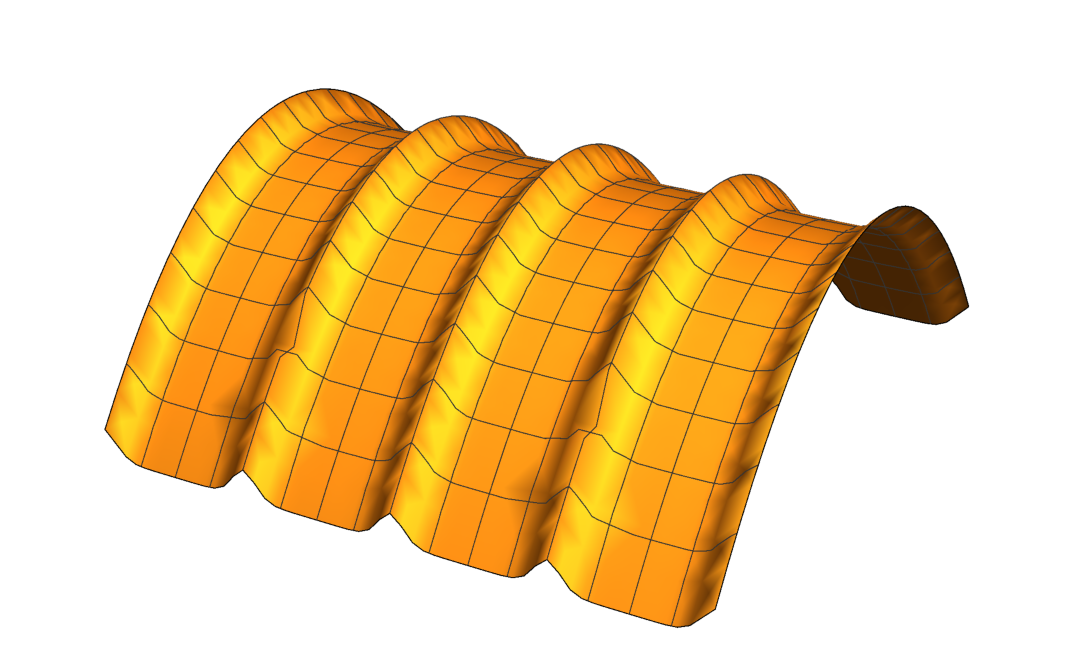
\includegraphics{./images/ch10/iUnD.pdf}}
\end{center}

{\bf 例:}设$F(x,y,z)$在条件$\varphi(x,y,z)=0$和$\psi(x,y,z)=0$
之下在点$P_0(x_0,y_0,z_0)$处取得极值$m$,证明:曲面
$F(x,y,z)=m,\varphi(x,y,z)=0$和$\psi(x,y,z)=0$
在$P_0$的法线共面,其中函数$F,\varphi,\psi$均有连续且不同时
为零的一阶偏导数。

{\bf 例:}求函数$z=x^2-xy+y^2$在区域$D:|x|+|y|\leq 1$
上的最大和最小值。

[提示]:令$x+y=X,x-y=Y$,则\ps{任意形如$ax^2+bxy+cy^2$的函数都可以通过
该线性变换化为形如$AX^2+BY^2$的形式!}
$$z=x^2-xy+y^2=\df14X^2+\df34Y^2,$$
$$D:|x|+|y|\leq 1\quad\Leftrightarrow\quad |X|\leq1,|Y|\leq1$$
易知$|X|=|Y|=1$时,$z$取最大值$1$,$|X|=|Y|=0$时,$z$取最大值$0$.

如果使用普通的方法,计算量会大很多。

\subsection*{课堂思考}

{\bf 例:}设$F(x,y)=\dint_0^{xy}\df{\sin t}{1+t^2}\d t$,则
$\left.\df{\p^2F}{\p x^2}\right|_{x=0 \atop y=2}=$
\underline{\quad\quad\quad}

{\bf 例:}设$z=f(xy,yg(x))$,其中$f$二阶偏导数连续,$g(x)$可导且
有极值$g(1)=1$,求$\left.\df{\p^2z}{\p x\p y}\right|_{x=1\atop y=1}$

\newpage

\section*{课后作业}
\addcontentsline{toc}{section}{课后作业}

{\bf 【必作题】}

\begin{itemize}
  \setlength{\itemindent}{1cm}
  \item 习题10.1:9(3,4),12,13
  \item 习题10.2:5(3,4),8,9,13,14,20
  \item 习题10.3:8,16,18,23,24,26,27
  \item 习题10.4:6,7,8,9,13
  \item 习题10.5:3,4,5,7,10,14,15
\end{itemize}

\bigskip

\hrule

\bigskip

{\bf 【思考题】}

\begin{itemize}
  \setlength{\itemindent}{1cm}
  \item 习题10.1:15
  \item 习题10.2:11,16,17,18
  \item 习题10.3:所有未布置的题目
  \item 习题10.4:12,14,15,16
  \item 习题10.5:16,17,18,19
\end{itemize}

{\it\b 如果能够在本章开课一周内搞定以下的所有题,可以免交
本章必作题!欢迎选作!}

\begin{enumerate}
  \setlength{\itemindent}{1cm}
  \item 证明以下函数可微,但偏导数不连续\ps{本章必须掌握的一类题}
  	$$
	f(x,y)=\left\{\begin{array}{ll}
	0 & ,(x,y)=(0,0)\\
	(x^2+y^2)\sin\df1{x^2+y^2}& ,else
	\end{array}\right.
	$$
  \item 设$f(x,y)$一阶偏导连续,$f(1,1)=1,f\,'_x(1,1)=2$,
	$f\,'_y(1,1)=3$,又$\varphi(x)=f(x,f(x,x))$,求
	\ps{考试中经常出但又容易作错的小题}
	$$\left.\df{\d\varphi^3(x)}{\d x}\right|_{x=1}$$
  \item 设$u=u(x,y,z)$具有连续偏导数,且\ps{基本的偏导数计算问题}
	$$x=r\sin\theta\cos\varphi,y=r\sin\theta\sin\varphi,z=r\cos\theta$$
	证明:若$x\df{\p u}{\p x}+y\df{\p u}{\p y}+z\df{\p u}{\p z}=0$,
	则$u$与$r$无关。
  \item 设$u=u(x,y,z)$,证明:$u$为$x,y,z$的线性函数,当且仅当
	$\bigtriangledown u$为常矢量。	\ps{正确叙述解题过程是关键!}
  \item 证明:当$x,y$很小时,$\arctan\df{x+y}{1+xy}\approx x+y$
  \item 求以$(0,0),(0,1),(1,0)$为顶点的三角形区域内
	到该三点距离平方和最大的点。\ps{基础题,必考!}
  \item 求函数$z=x^2-xy+y^2$在区域$D:|x|+|y|\leq 1$
	上的最大和最小值。\ps{基础题,必考!}
  \item 在半径为$R$的圆的内接三角形中,求面积最大者。\ps{基础题,必考!}
  \item 设$F(x,y,z)$在条件$\varphi(x,y,z)=0$和$\psi(x,y,z)=0$
	之下在点$P_0(x_0,y_0,z_0)$处取得极值$m$,证明:曲面
	$F(x,y,z)=m,\varphi(x,y,z)=0$和$\psi(x,y,z)=0$
	在$P_0$的法线共面,其中函数$F,\varphi,\psi$均有连续且不同时
	为零的一阶偏导数。
\end{enumerate}

\newpage

\section*{习题参考解答}
\addcontentsline{toc}{section}{习题参考解答}

{\bf 习题10.1}

9.(3)\;解:
$$
	\lim\limits_{(x,y)\to(0,0)}\df{2-\sqrt{xy+4}}{xy}
	=\lim\limits_{(x,y)\to(0,0)}\df{-xy}{xy\left(2+\sqrt{xy+4}\right)}
	=-\df14
$$

(4)\;解:
$$
	\lim\limits_{(x,y)\to(2,0)}\df{\sin(xy)}{y}
	=\lim\limits_{(x,y)\to(2,0)}\df{xy}{y}
	=\lim\limits_{(x,y)\to(2,0)}x=2
$$

12.(1)\;证:因为
$$
	\lim\limits_{x\to 0\atop{y=kx}}\df{x+y}{x-y}
	=\lim\limits_{x\to 0\atop{y=kx}}\df{x+kx}{x-kx}=\df{1+k}{1-k},
$$
结果与$k$有关,这说明当自变量沿不同方向趋于$(0,0)$时,函数有不同极限,所以
原二重极限不存在。

(2)\;证:因为
$$
	\lim\limits_{x\to 0\atop{y=kx}}\df{\ln(1+xy)}{x(x+y)}
	=\lim\limits_{x\to 0\atop{y=kx}}\df{xy}{x(x+y)}
	=\lim\limits_{x\to 0\atop{y=kx}}\df{kx^2}{(1+k)x}=\df{k}{1+k},
$$
结果与$k$有关,这说明当自变量沿不同方向趋于$(0,0)$时,函数有不同极限,所以
原二重极限不存在。

13.(1)\;解:设$x=\rho\cos\theta,y=\rho\sin\theta$,则
$$
	\lim\limits_{(x,y)\to(0,0)}\df{3x^2-x^2y^2+y^2}{x^2+y^2}
	=3\cos^2\theta+\sin^2\theta,
$$
结果与$\theta$有关,故$f(x,y)$当$(x,y)\to(0,0)$时极限不存在,从而无论
如何定义$f(0,0)$,函数$f(x,y)$都不可能在$(0,0)$处连续。

(2)\;解:设$x=\rho\cos\theta,y=\rho\sin\theta$,则
$$
	\lim\limits_{(x,y)\to(0,0)}=\lim\limits_{\rho\to0}
	2\rho\cos\theta\sin^2\theta=0,
$$
由此可知,令$f(0,0)$即可。

{\bf 习题10.2}

5.(3)\;解:
$$z''_{xx}=\df{-2x}{(1+x^2)^2},\quad
z''_{yy}=\df{-2y}{(1+y^2)^2}\quad
z''_{xy}=0.$$

(4)\;解:
\begin{align*}
	z''_{xx}&=y^x\ln^2y\ln(xy)+\df{2y^x\ln y}x-\df{y^x}{x^2}\\
	z''_{yy}&=x(x-1)y^{x-2}\ln(xy)+2xy^{x-2}-y^{x-2}\\
	z''_{xy}&=xy^{x-1}\ln y\ln(xy)+y^{x-1}\ln(xy^2)+y^{x-1}
\end{align*}

8.\;(1)$\d f=e^{\frac{\sin y}x}\df1{x^2}\cos\df yx(x\d y-y\d x)$

(2)$\d f=e^x(\sin y+\cos y+x\sin y)\d x+e^x(-\sin y+x\cos y)\d y$

(3)$\d f=x^{y^2z}\left(\df{y^2z}x\d x+2yz\ln x\d y+y^2\ln x\d z\right)$

(4)$\d f=\df{xyz}{1+(xyz)^2}\left(\df{\d x}x+\df{\d y}y+\df{\d z}z\right)$

9.\;$\df13\d x+\df23\d y$

13.\;$\df12x^2+y^2\ln x+\sin y-\df12$

14.\;$z'_x=-e^{-x^2},\;z'_y=2e^{-4y^2}$

15.\;解:设圆锥的地面半径和高分别为$r,h$,则其体积$V=\df13\pi r^2h$,进而
$$\Delta V\approx\d V=\df23\pi rh\d r+\df13\pi r^2\d h\leq 20\pi,$$
也即计算圆锥体积的最大误差为$20\pi(\mathrm{cm}^3)$

{\bf 习题10.3}

8.$-1$

16.\;切线:$\df{x+2}{25}=\df{y-1}{28}=\df{z-6}{12}$,
法平面:$25x+28y+12z-50=0$.

18.$f'_y(x,2x)=x-\df12x^3$.

23.\;(1)$-2$;(2)$-1$.

24.\;$\varphi(1)=1,\;\varphi'(1)=a+ab+ab^2+b^3$,提示:
$$
	\varphi'(x)=f'_1(x,f(x,f(x,x)))+f'_2(x,f(x,f(x,x)))\left\{
	f'_1(x,f(x,x))+f'_2(x,f(x,x))[f'_1(x,x)+f'_2(x,x)]\right\}
$$

26.\;(2)[提示]:$xz'_x-yz'_y=xf(u)+\df{x^2}yf(u)$,代入方程可得
$$f(u)+2uf'(u)=0\quad\Rightarrow\quad f(u)=-Cu^{-1/2}\;(C\in\mathbb{R})$$

27.\;$f(u)=C_1e^u+C_2e^{-u},\;(C_1,C_2\in\mathbb{R})$

{\bf 习题10.4}

6.\;$5+2(x-1)^2-(x-1)(y+2)-(y+2)^2$

7.\;$y+xy-\df12y^2+\circ(x^2+y^2)$

8.\;$\df{\sqrt2}3$

9.\;$\sqrt2\df{\sqrt{a^2+b^2}}{ab}$

{\bf 习题10.5}

3.\;在$\left(\df{18}{13},\df{12}{13}\right)$处取极小值$\df{36}{13}$

4.\;$\df{100}{3}\left(1,1,1\right)$

5.\;最大值$z(-3,4)=125$,最小值$z(3,-4)=75$

7.\;最小值点$\left(\df12,\df14\right)$,最小值$\df{7\sqrt2}8$

10.\;最大值$z(-1,1)=5$,最小值$z(1,-1)=-5$

15.\;从距离两边各$8\mathrm{cm}$处折起,腰与底边夹角为$\df{\pi}3$时断面面积最大

\ifvisible

\section*{关于评教}

{\it (以下都是我特别想了解的问题,欢迎大家结合自己的感受发表宝贵的意见,提出改进的建议)}

\begin{enumerate}
  \item 关于课堂
  \begin{itemize}
    \item 我们目前授课的节奏,你觉得合适吗?进度是否太快,或者,太慢?
    \item 关于我上课的方式和课堂讲解,你觉得自己的接受程度如何?我哪方面特别需要改进?
    \item 多媒体演示还需要多一些吗?你觉得怎样能使演示的效率更高、效果更好? 
    \item 有必要继续安排课前写题吗?每次讲评总是会占用一部分正课时间,有没有其他好的解决办法?
  \end{itemize}
  \item 关于作业与练习
  \begin{itemize}
    \item 作业量是否过多?难度合适吗?
    \item 对目前采取的作业批改方式,你觉得效果如何,有没有什么改进的方法?
    \item 对于我批改的作业以及作业评分,你感觉满意吗?有什么具体的意见和建议?
    \item 你个人课后看书、作作业以及看辅导资料的时间充足吗?
    \item 能不能估算出一周除了上课,你自己大概还有多少时间花在了和高数有关的事情上?
    能否把估算的结果告诉我?
  \end{itemize}
  \item 关于交流与讨论
  \begin{itemize}
    \item 微信群和云盘这样的交流平台,你觉得真的有效果吗?你有没有下载过云盘上的资料?
    \item 你觉得老师和学生之间应该用什么样的方式来讨论问题?
    \item 我们有必要安排定期的答疑吗?最长多少时间合适呢?
  \end{itemize}
  \item 其他任何与我们这门课和我个人教学有关的意见和建议
\end{enumerate}

\fi

% \newpage
% 
% {\bf 第10章习题课作业}
% 
% {\it 本次作业请抄题!}



